% !Mode:: "TeX:UTF-8"

\section{功能展示}

\subsection{功能描述}

\subsubsection{实验05基础功能}

实验05实现上位机控制HDMI显示模式，支持：
\begin{itemize}
    \item 原图显示（mode=0）
    \item 灰度图显示（mode=1）
    \item Sobel边缘检测（mode=2）
    \item 彩色边缘叠加（mode=3）
    \item 阈值调整（0-255）
\end{itemize}

\subsubsection{综合扩展任务3完成情况}

新增3种边缘检测算法（Prewitt、Laplacian、Roberts），实现：
\begin{itemize}
    \item 新增PL图像处理算法：3个核心模块
    \item 显示模式选择命令：mode=4/5/6选择新算法
    \item 软件golden output：Python生成4种算法参考输出
    \item RTL仿真验证：仿真模型通过所有测试
    \item 资源利用率与性能：Vivado综合结果
\end{itemize}

\subsection{演示结果}

\subsubsection{仿真验证结果}

RTL仿真验证显示控制模型，覆盖7种显示模式。所有模式二值化逻辑正确验证，阈值比较功能正常。

\begin{figure}[H]
    \centering
    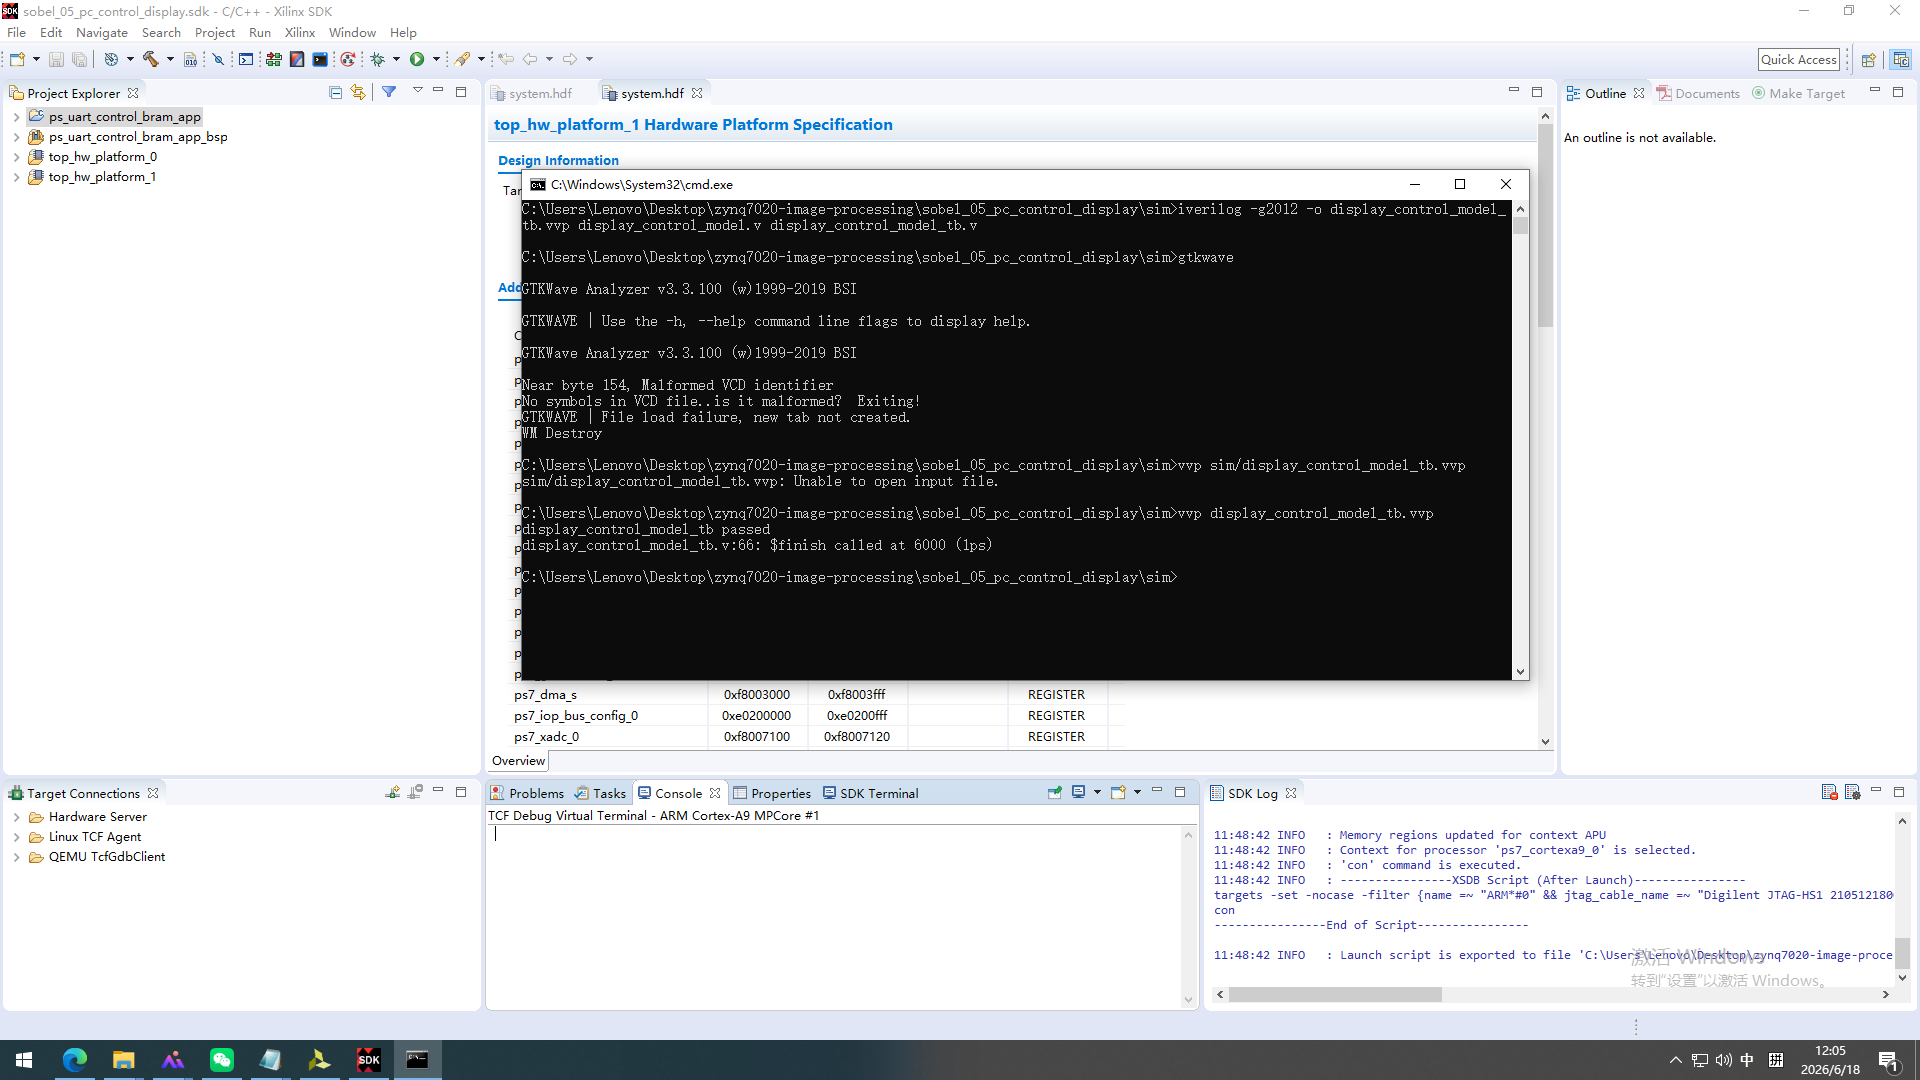
\includegraphics[width=0.9\textwidth]{images/05/仿真通过.png}
    \caption{显示控制模型仿真通过}
    \label{fig:sim_pass}
\end{figure}

如图\ref{fig:sim_pass}所示，仿真测试全部通过，验证了各模式下的显示逻辑正确性。

\begin{figure}[H]
    \centering
    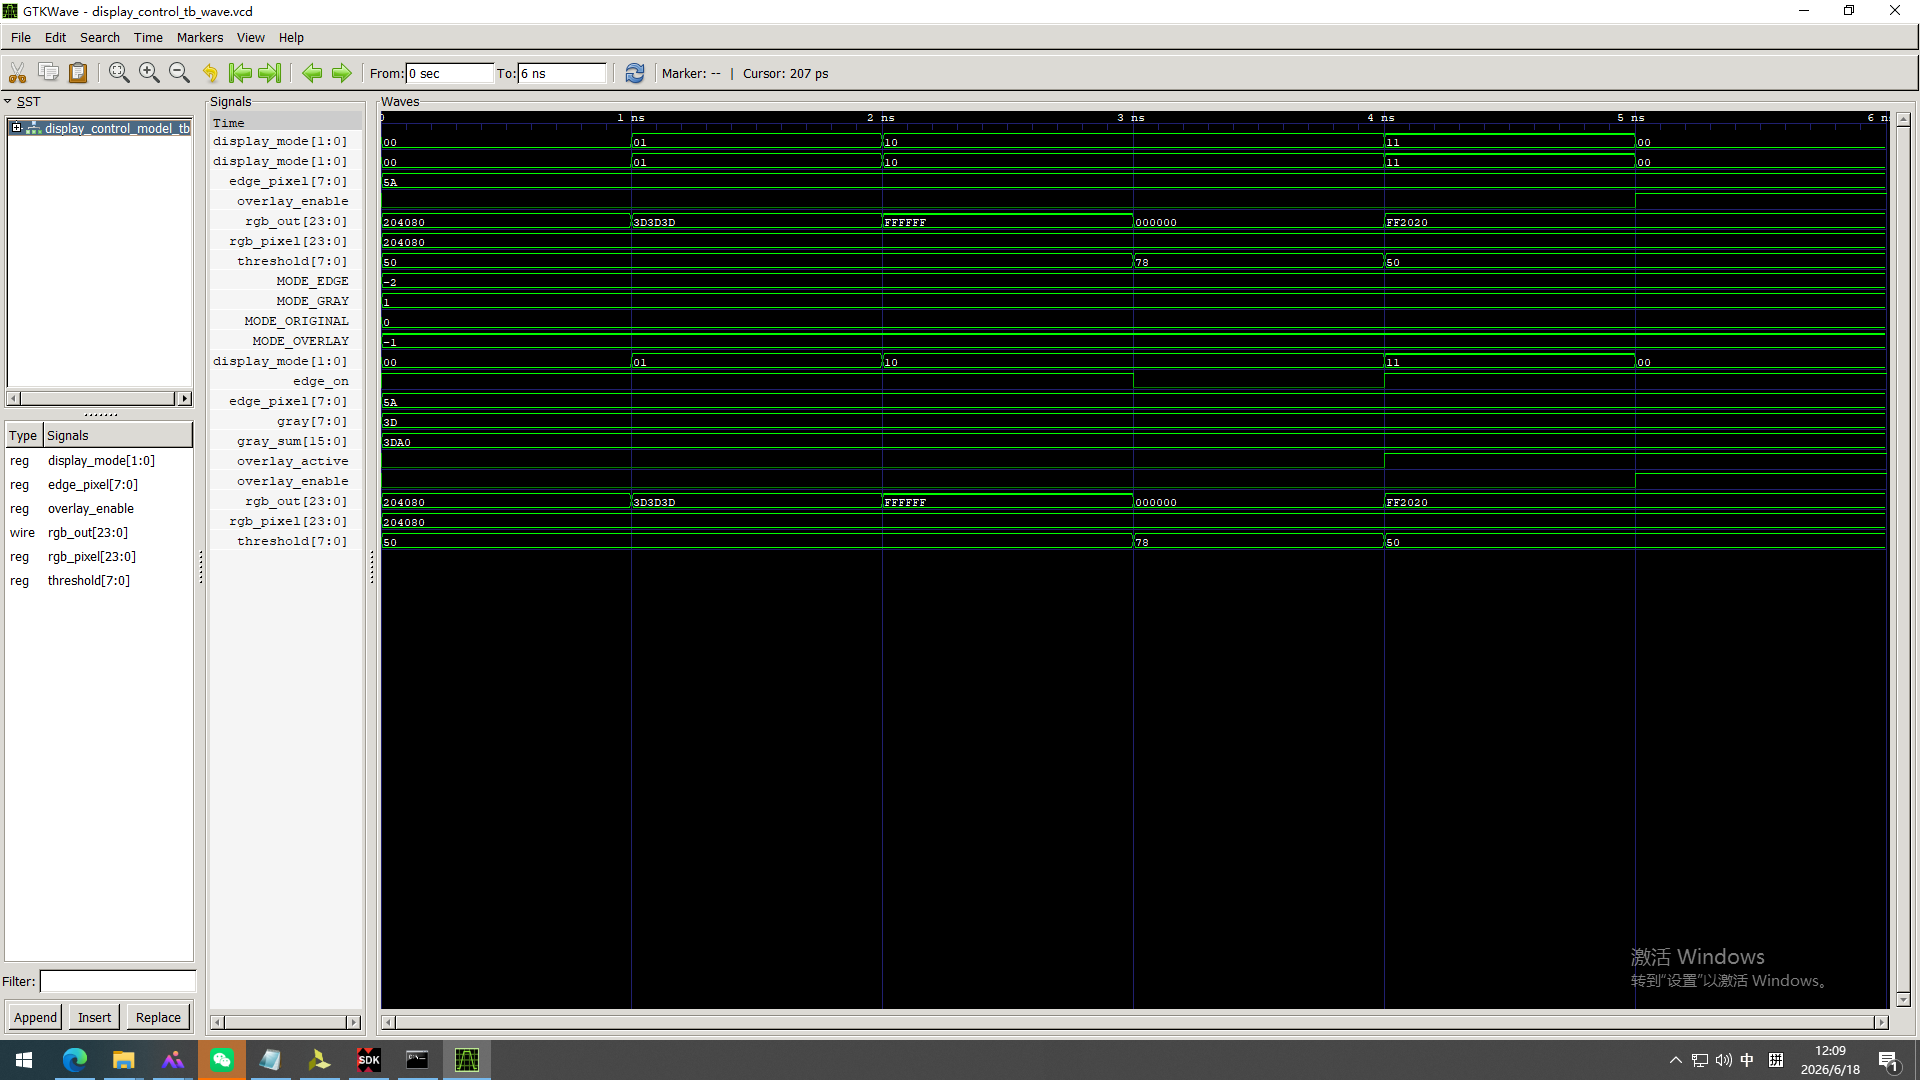
\includegraphics[width=0.9\textwidth]{images/05/仿真波形.png}
    \caption{显示控制模型仿真波形}
    \label{fig:sim_wave}
\end{figure}

如图\ref{fig:sim_wave}展示了关键信号的时序波形，包括display\_mode切换、edge\_data阈值比较和RGB输出。

\subsubsection{软件Golden Output对比}

使用Python生成4种算法的参考输出，对比如图\ref{fig:golden1}和\ref{fig:golden2}所示。

\begin{figure}[H]
    \centering
    \begin{minipage}{0.48\textwidth}
        \centering
        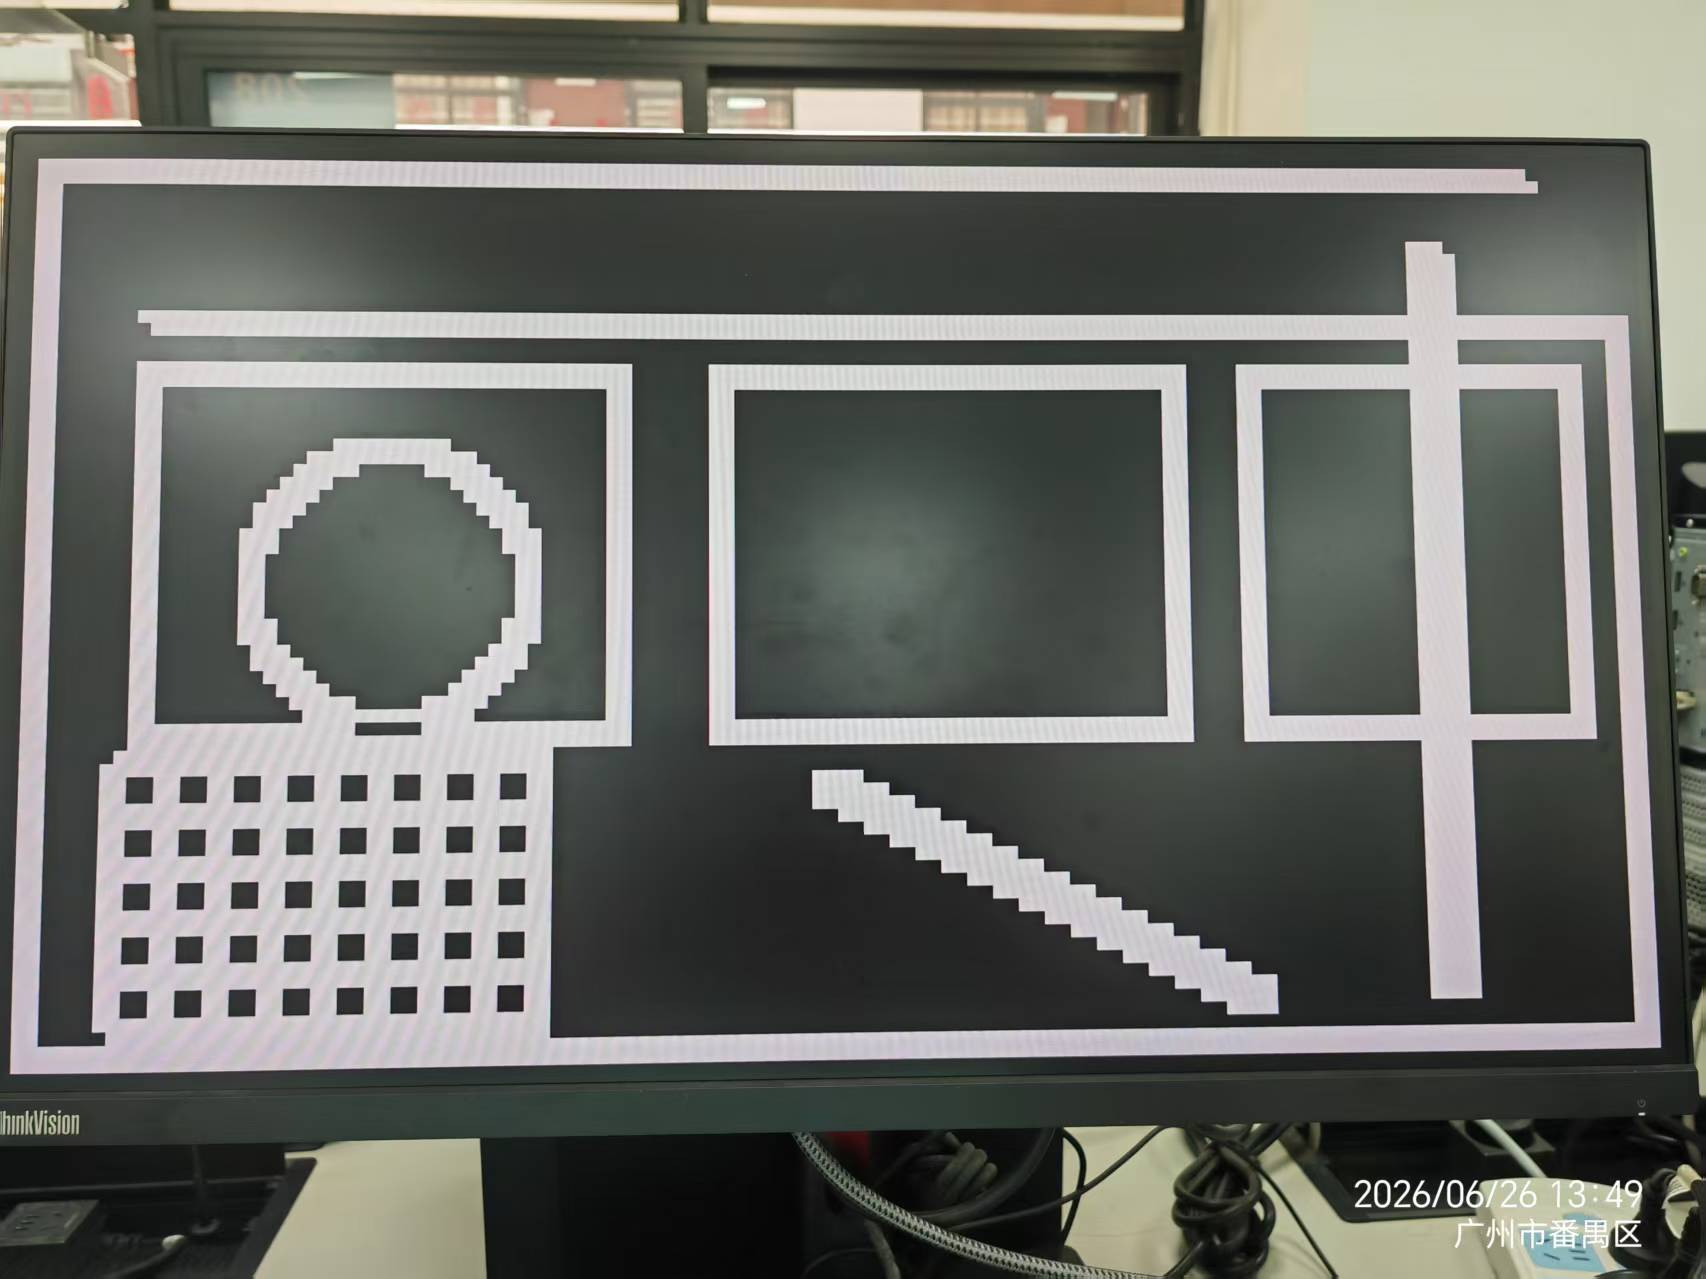
\includegraphics[width=\linewidth]{images/05扩展3/sobel_golden.jpg}
        \caption{Sobel}
    \end{minipage}
    \hfill
    \begin{minipage}{0.48\textwidth}
        \centering
        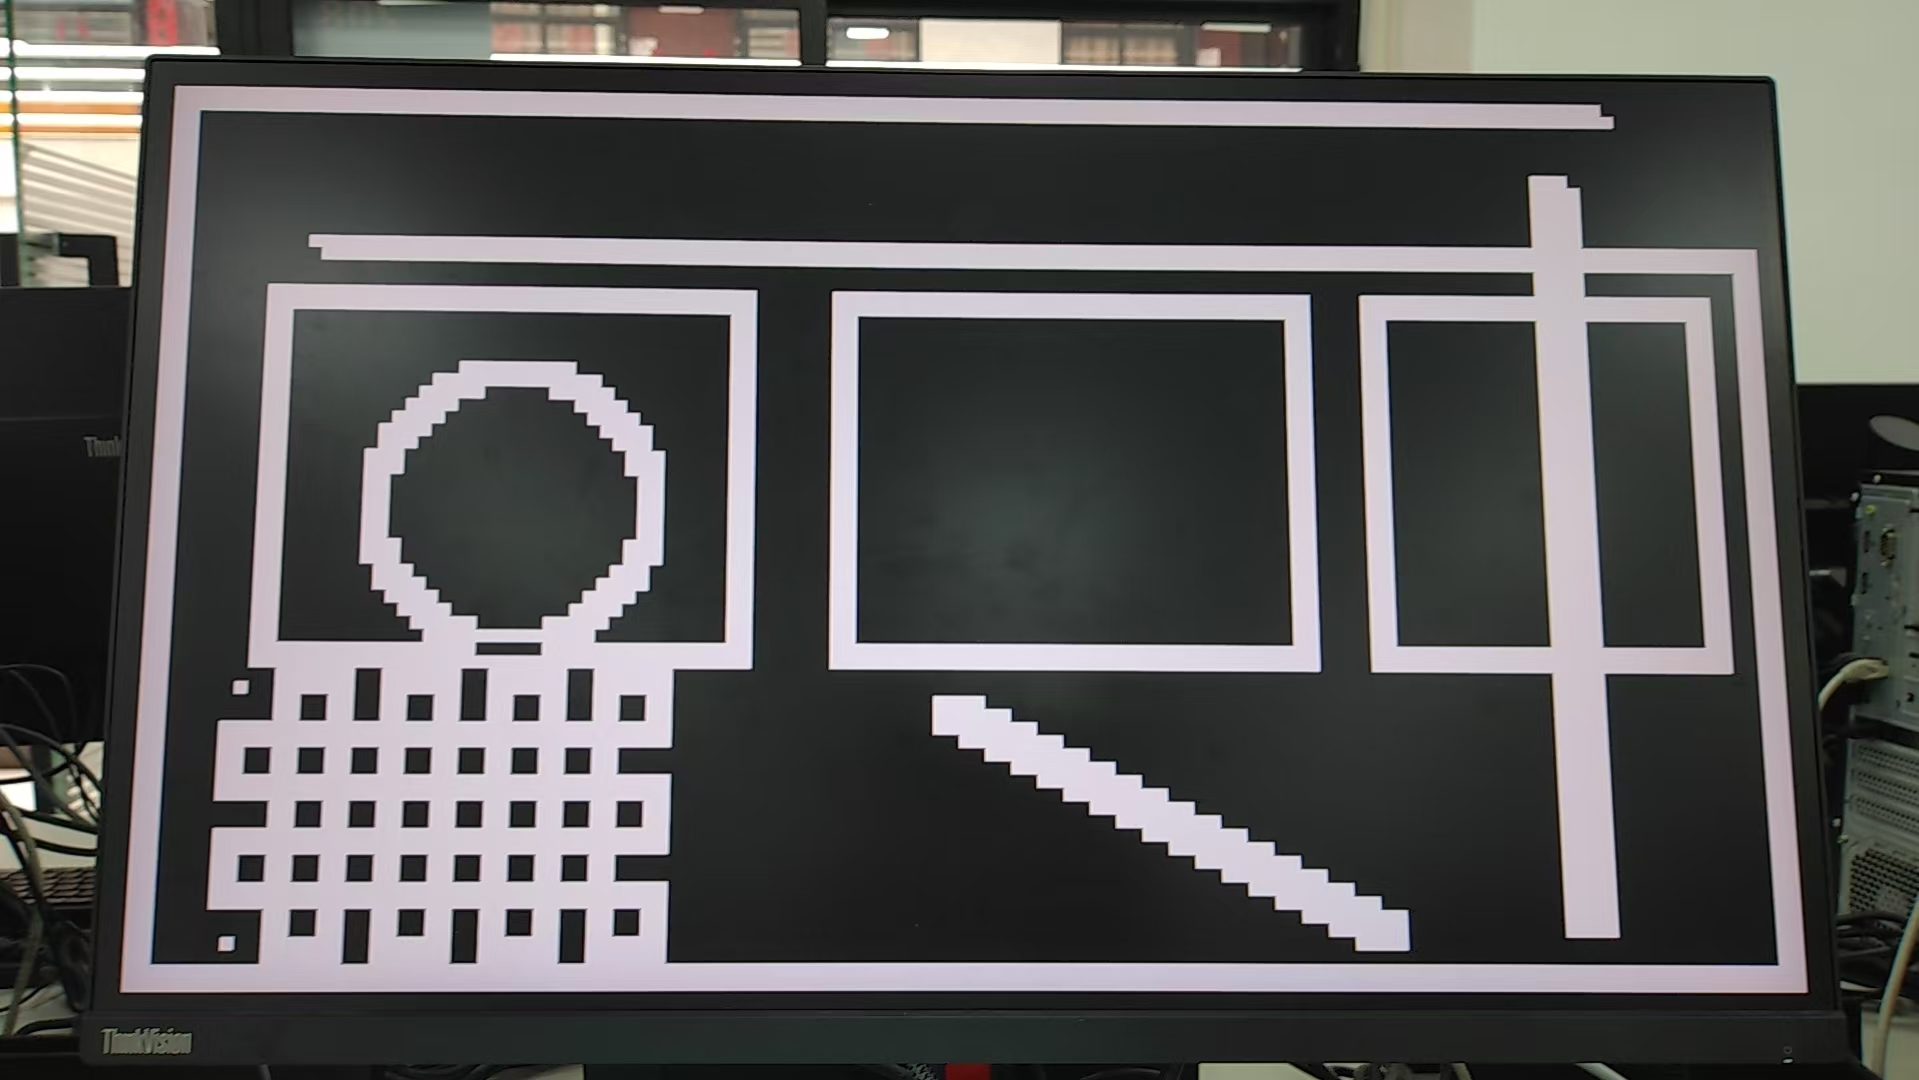
\includegraphics[width=\linewidth]{images/05扩展3/prewitt_golden.jpg}
        \caption{Prewitt}
    \end{minipage}
    \caption{Sobel与Prewitt Golden Output对比}
    \label{fig:golden1}
\end{figure}

从图\ref{fig:golden1}中可以观察到：Sobel算法边缘响应最均衡，对水平和垂直边缘都有较好的检测效果；Prewitt算法由于去掉了2x中心权重，边缘响应整体较弱，但边缘更平滑。

\begin{figure}[H]
    \centering
    \begin{minipage}{0.48\textwidth}
        \centering
        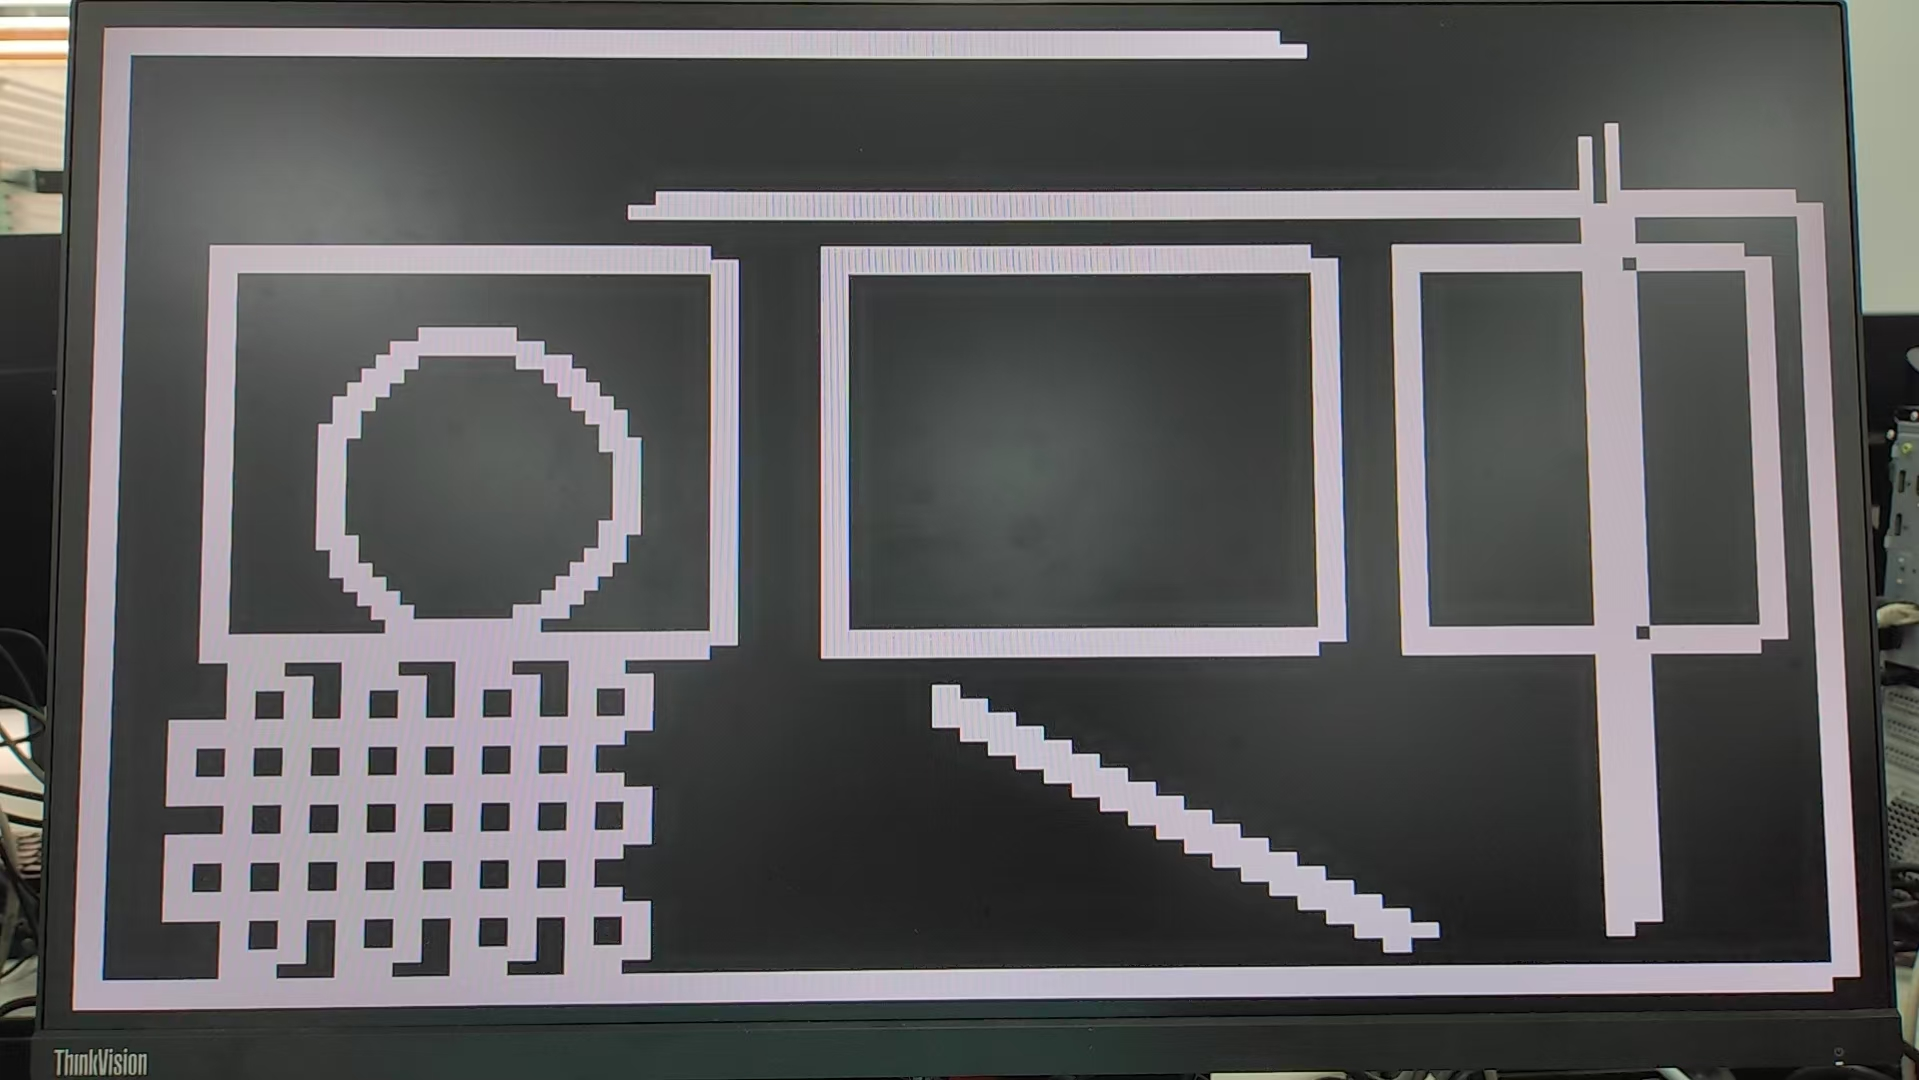
\includegraphics[width=\linewidth]{images/05扩展3/laplacian_golden.jpg}
        \caption{Laplacian}
    \end{minipage}
    \hfill
    \begin{minipage}{0.48\textwidth}
        \centering
        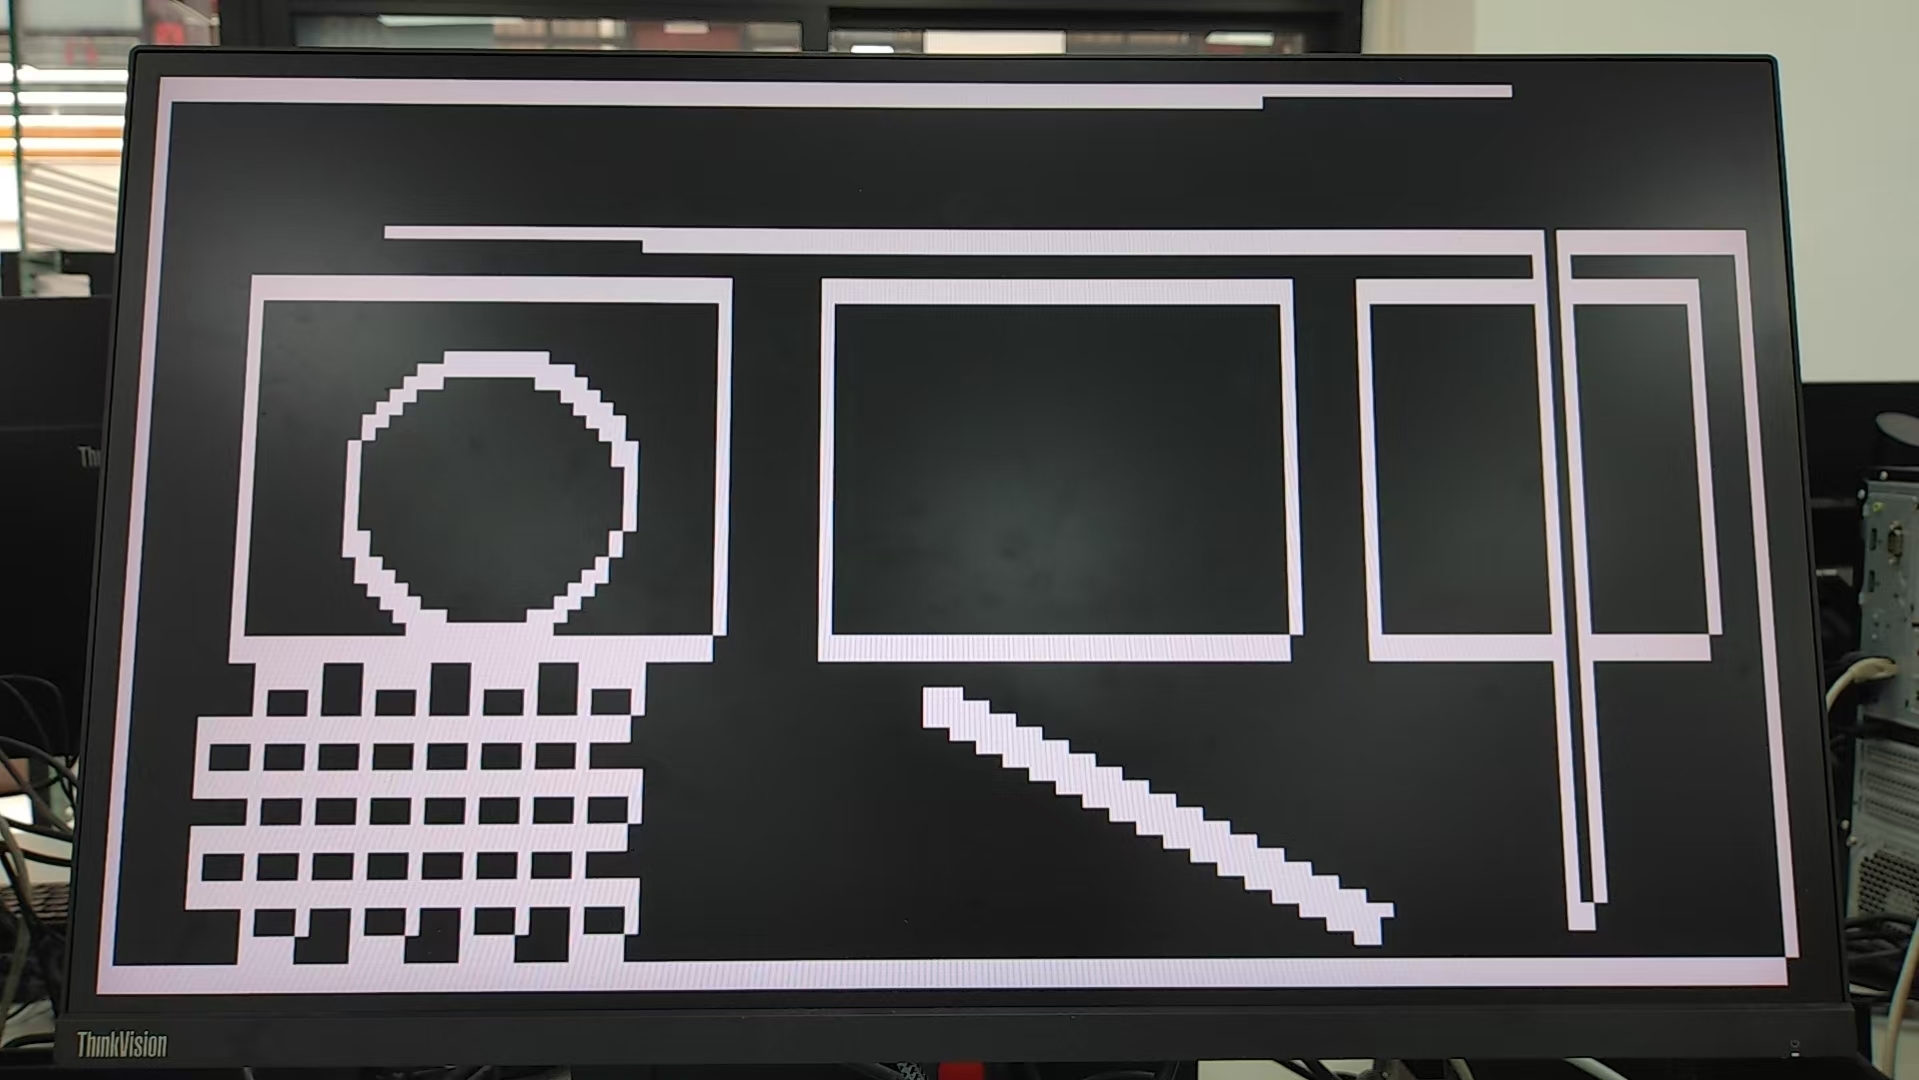
\includegraphics[width=\linewidth]{images/05扩展3/Robert_golden.jpg}
        \caption{Roberts}
    \end{minipage}
    \caption{Laplacian与Roberts Golden Output对比}
    \label{fig:golden2}
\end{figure}

从图\ref{fig:golden2}中可以观察到：Laplacian作为二阶导数算子，边缘细节最丰富，但对噪声也更敏感；Roberts使用2×2小卷积核，边缘响应较强，适合检测对角线方向的边缘。

\subsubsection{不同阈值对比}

在阈值40、60、80下对比四种算法的边缘检测结果。

\begin{figure}[H]
    \centering
    \begin{minipage}{0.48\textwidth}
        \centering
        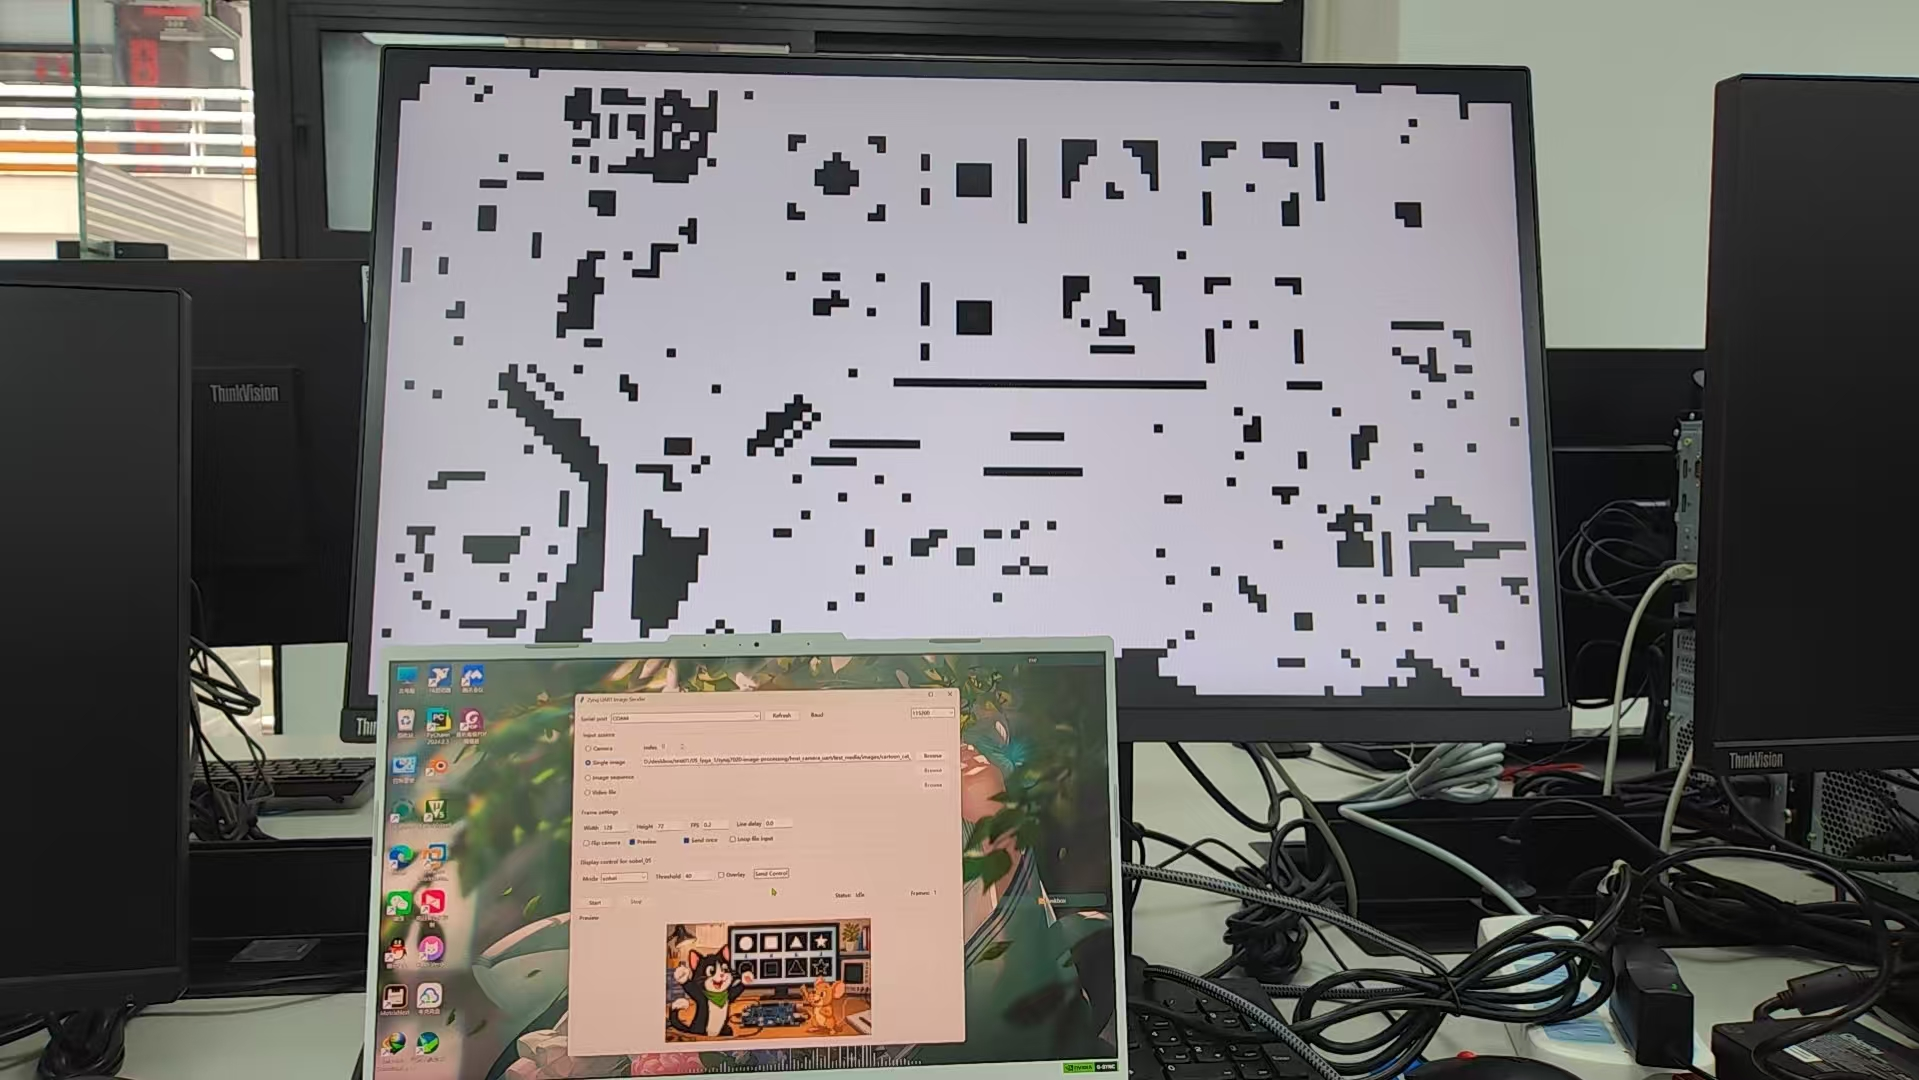
\includegraphics[width=\linewidth]{images/05扩展3/sobel_40.jpg}
        \caption{Sobel}
    \end{minipage}
    \hfill
    \begin{minipage}{0.48\textwidth}
        \centering
        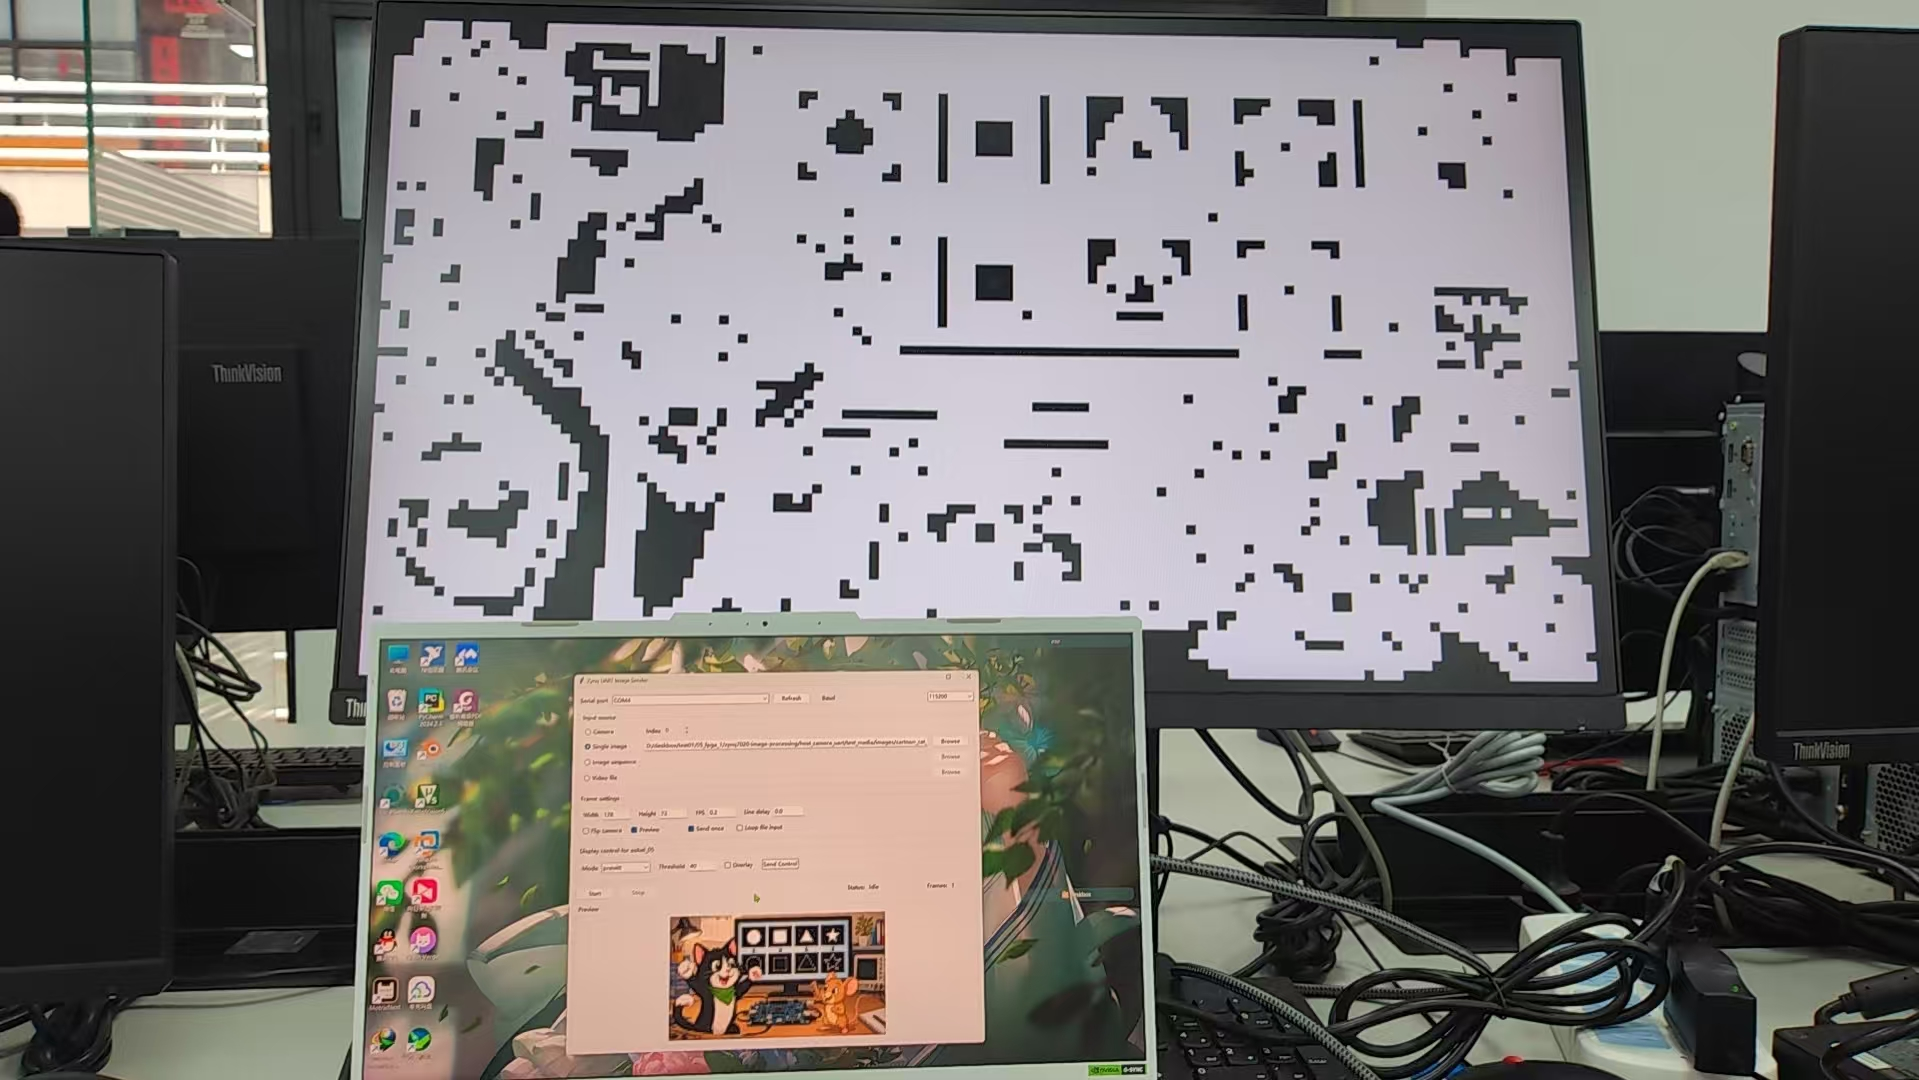
\includegraphics[width=\linewidth]{images/05扩展3/prewitt_40.jpg}
        \caption{Prewitt}
    \end{minipage}
    \par\vspace{1em}
    \begin{minipage}{0.48\textwidth}
        \centering
        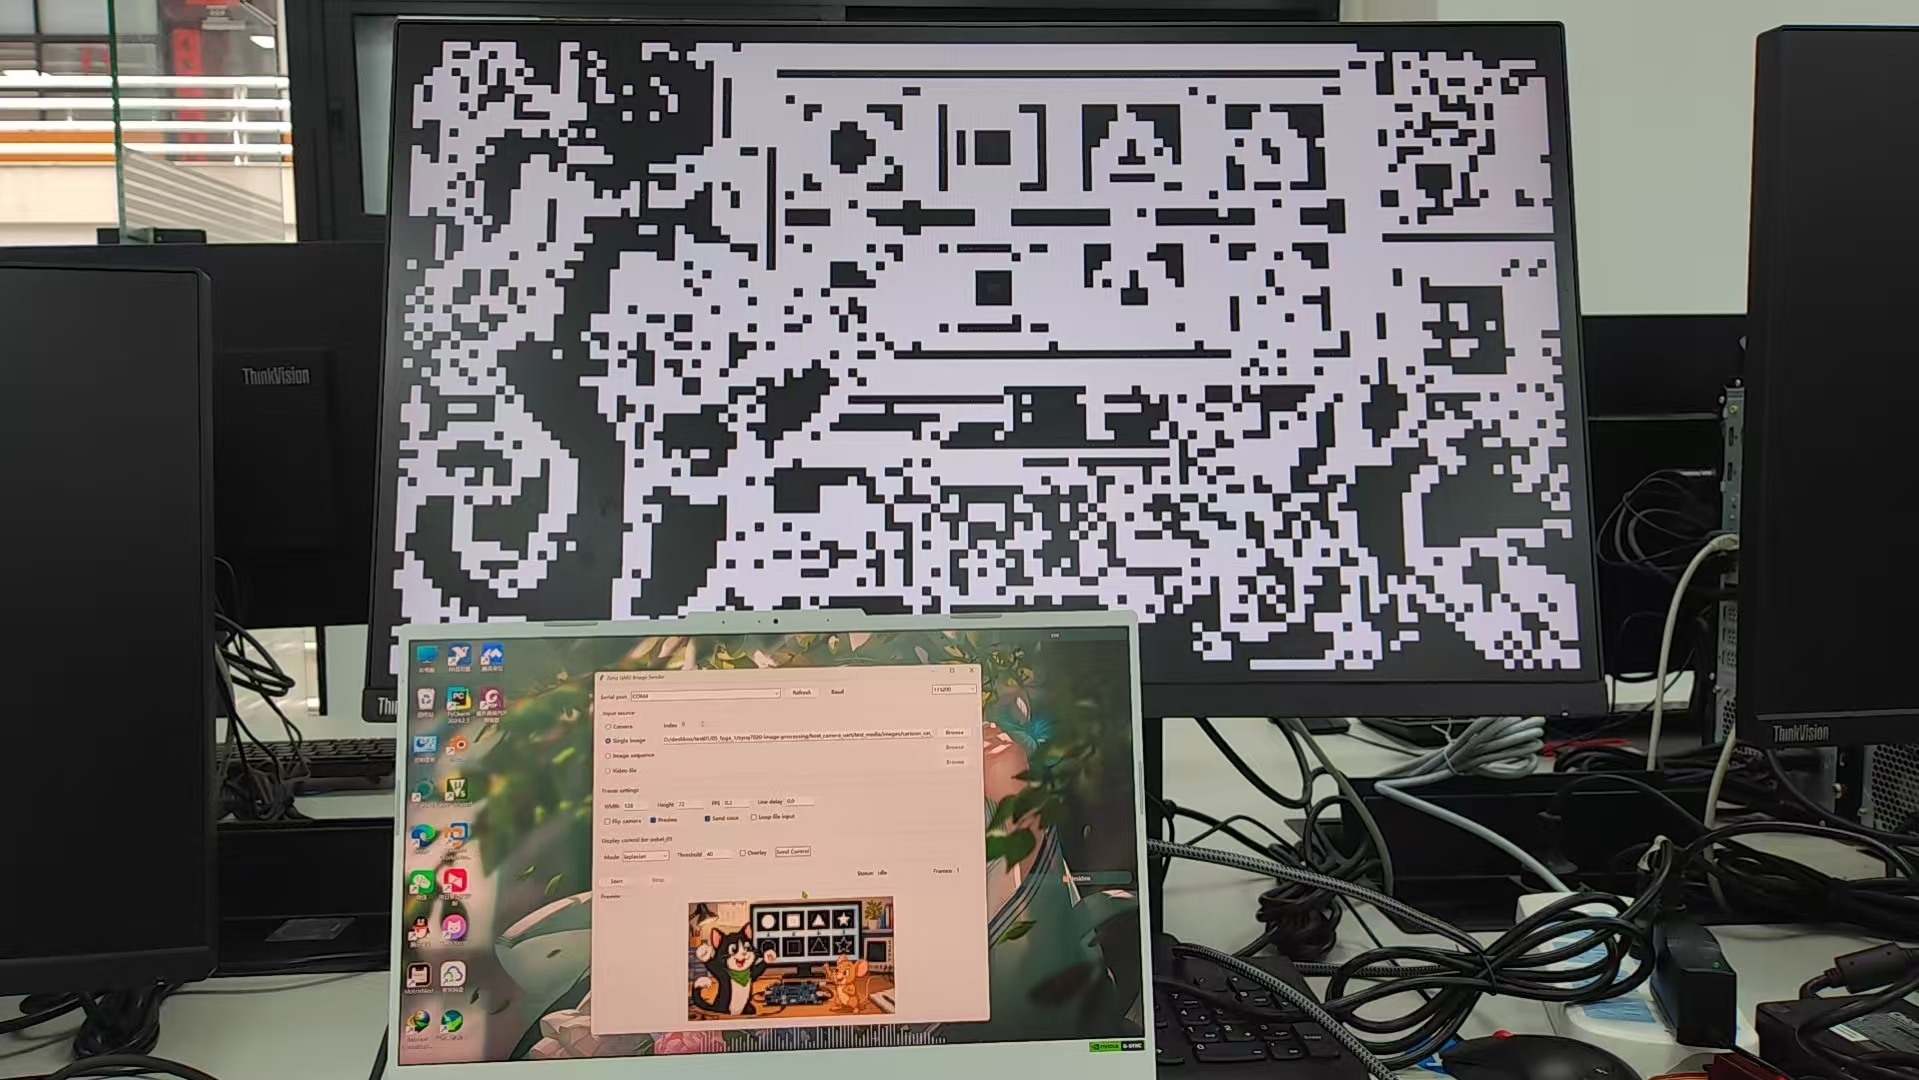
\includegraphics[width=\linewidth]{images/05扩展3/laplacian_40.jpg}
        \caption{Laplacian}
    \end{minipage}
    \hfill
    \begin{minipage}{0.48\textwidth}
        \centering
        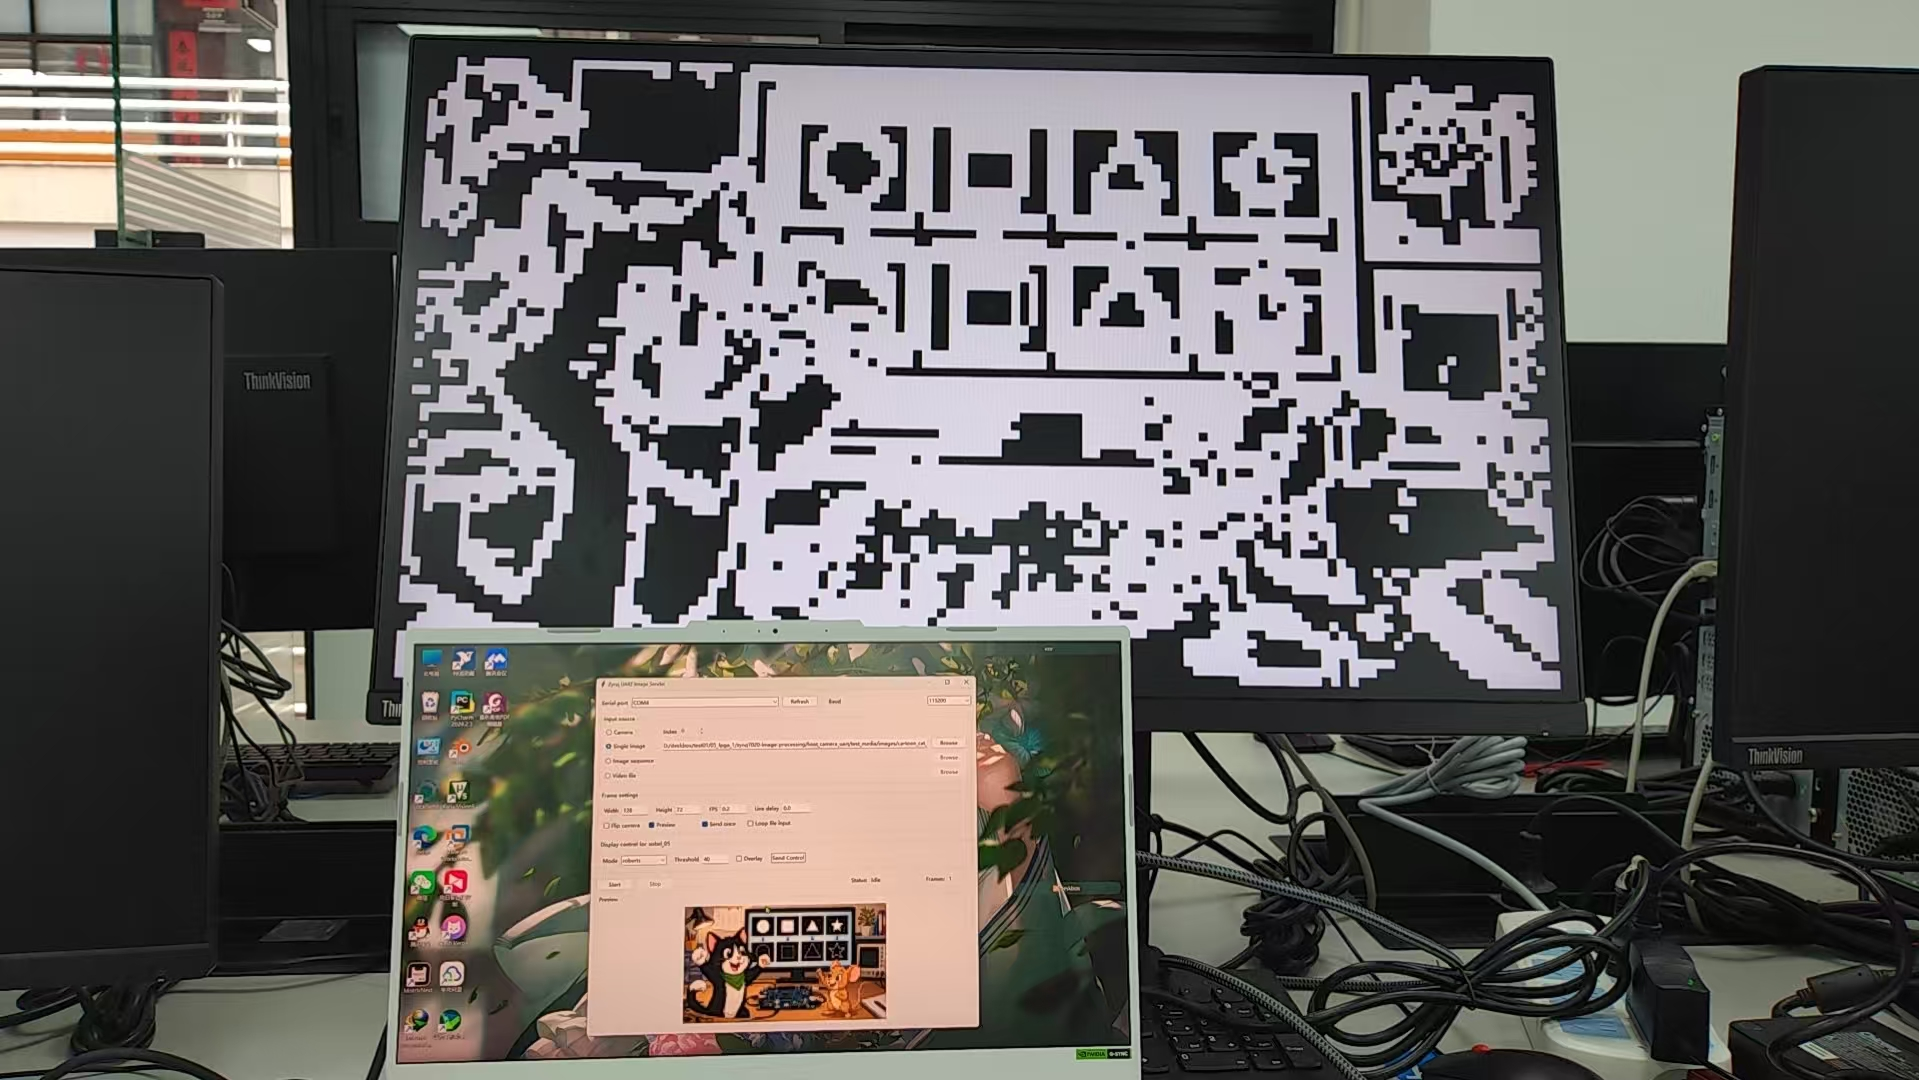
\includegraphics[width=\linewidth]{images/05扩展3/Robert_40.jpg}
        \caption{Roberts}
    \end{minipage}
    \caption{阈值40时四种算法对比}
    \label{fig:thresh40}
\end{figure}

如图\ref{fig:thresh40}所示，当阈值为40时，四种算法都检测到较多边缘。Sobel和Prewitt的边缘效果较为均衡，适合通用场景；Laplacian的边缘细节最丰富，但噪点也最多；Roberts的边缘响应较强，适合检测对角线方向的边缘。

\begin{figure}[H]
    \centering
    \begin{minipage}{0.48\textwidth}
        \centering
        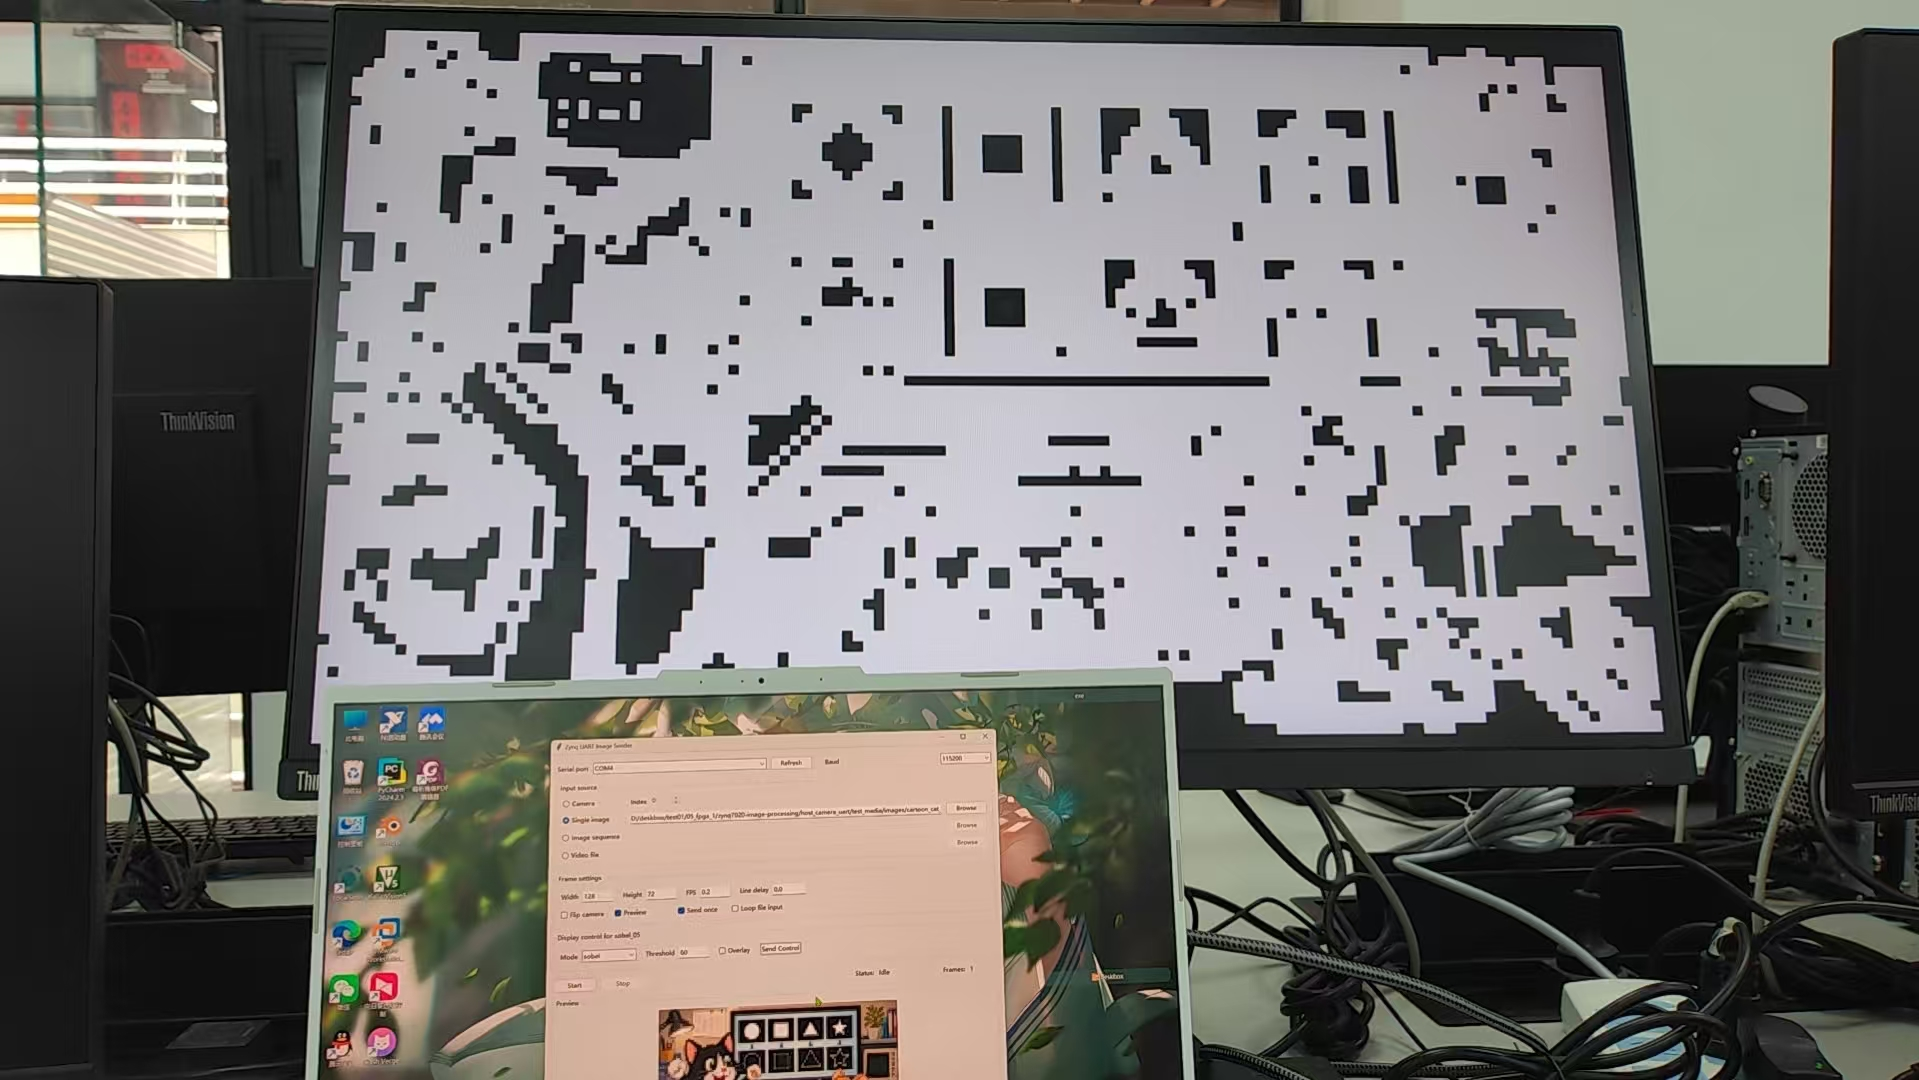
\includegraphics[width=\linewidth]{images/05扩展3/sobel_60.jpg}
        \caption{Sobel}
    \end{minipage}
    \hfill
    \begin{minipage}{0.48\textwidth}
        \centering
        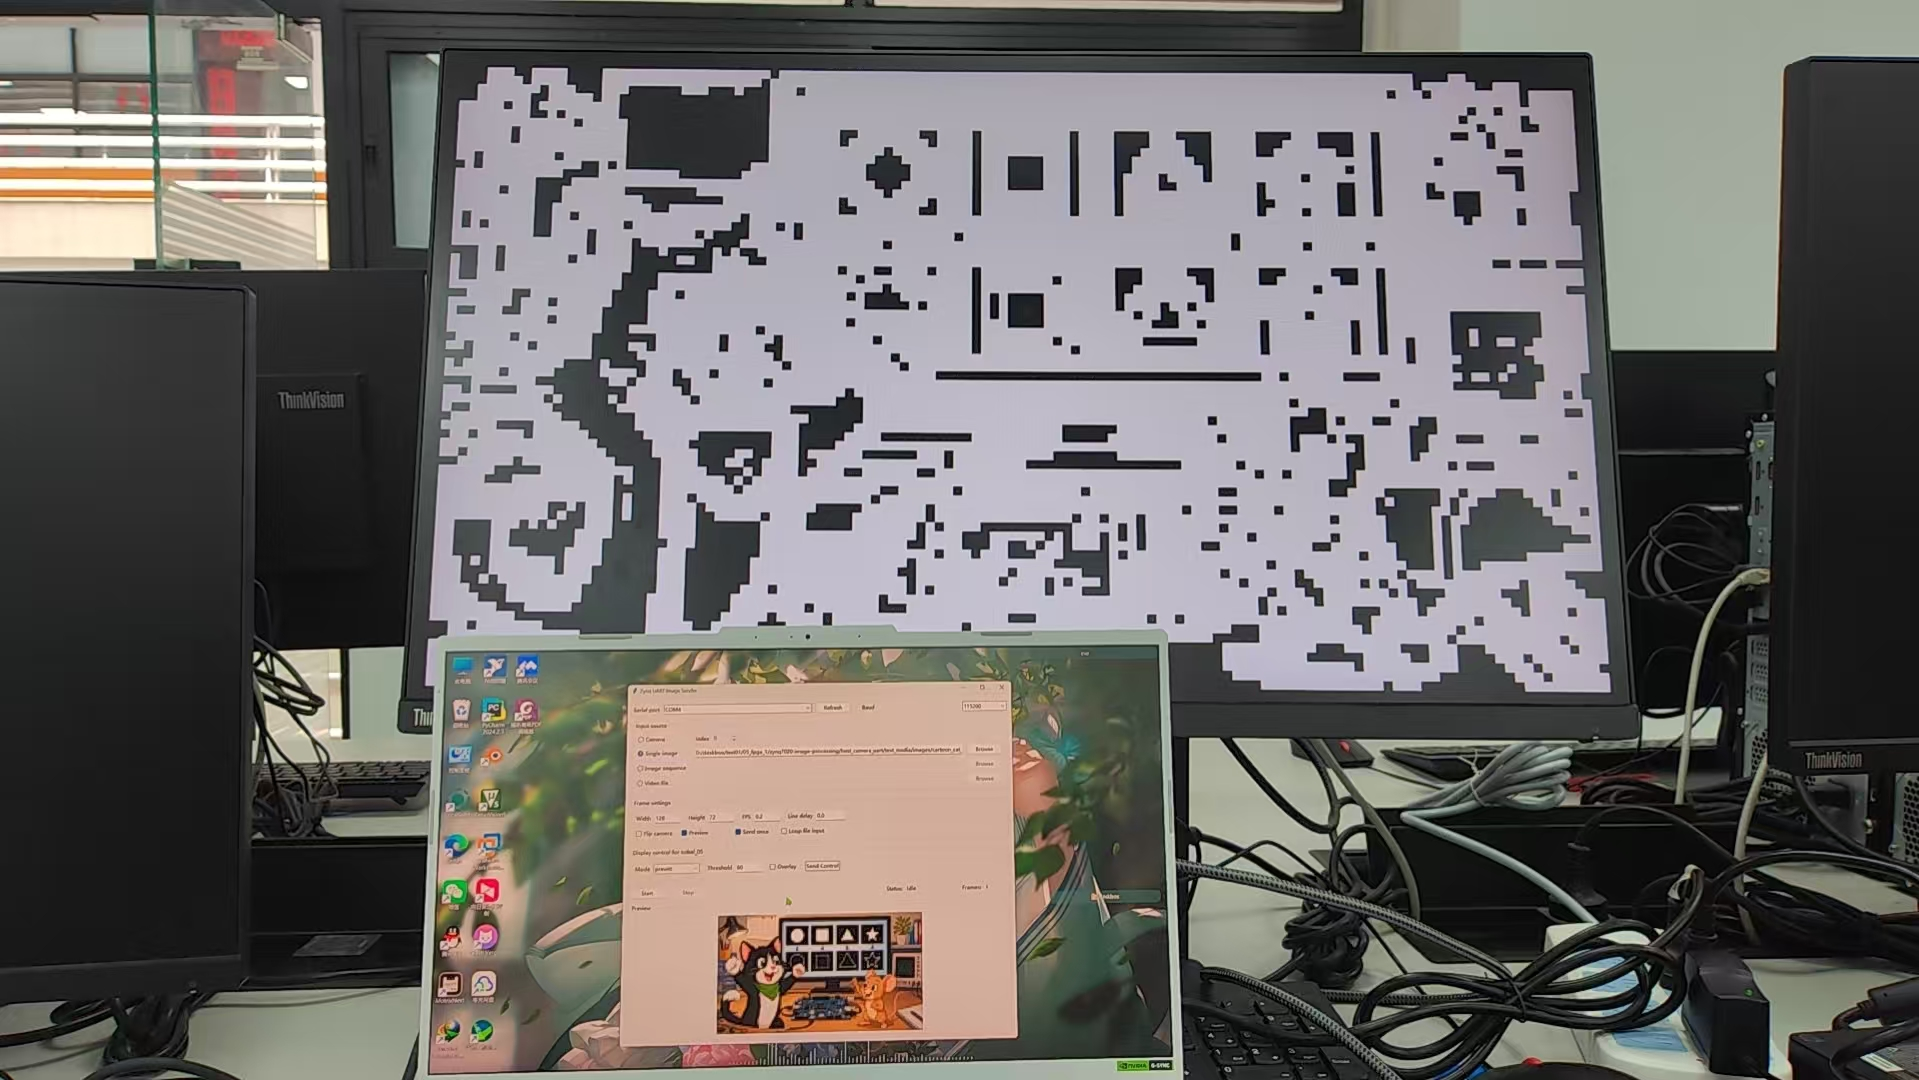
\includegraphics[width=\linewidth]{images/05扩展3/prewitt_60.jpg}
        \caption{Prewitt}
    \end{minipage}
    \par\vspace{1em}
    \begin{minipage}{0.48\textwidth}
        \centering
        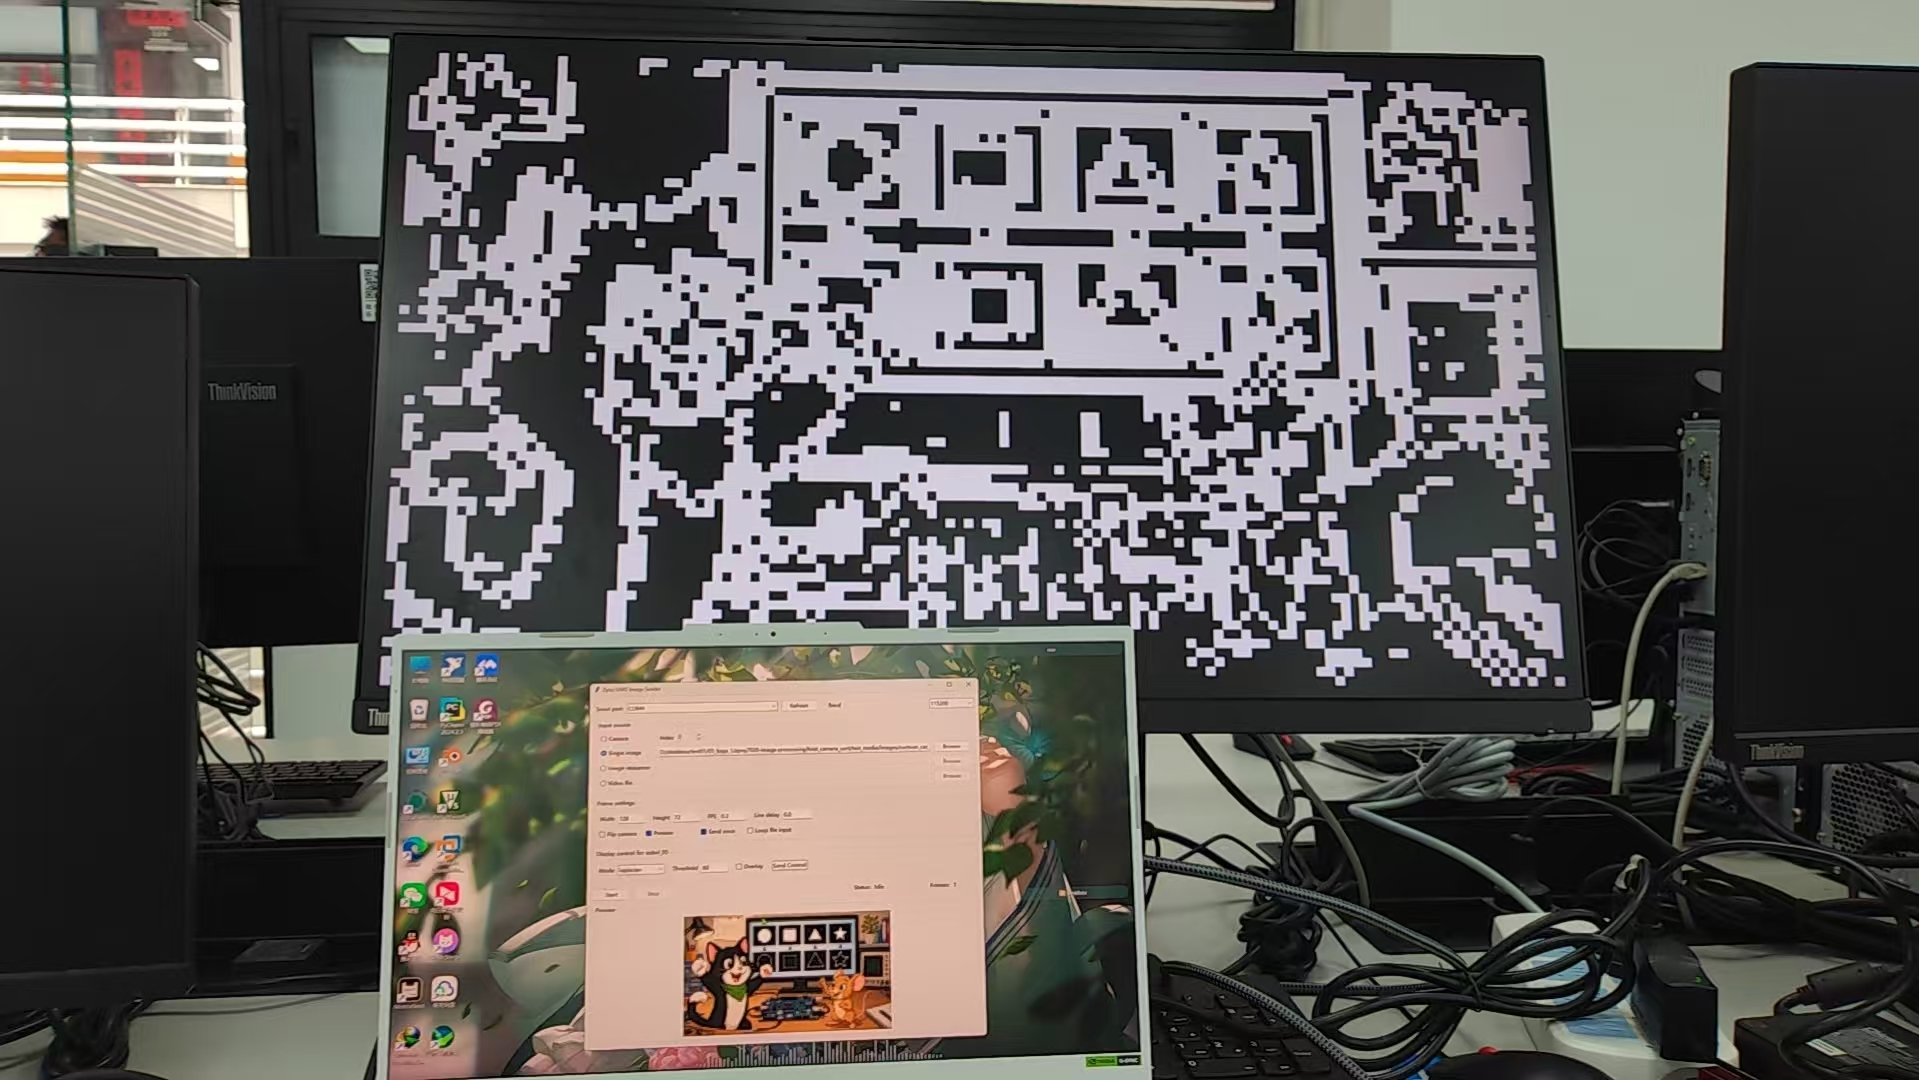
\includegraphics[width=\linewidth]{images/05扩展3/laplacian_60.jpg}
        \caption{Laplacian}
    \end{minipage}
    \hfill
    \begin{minipage}{0.48\textwidth}
        \centering
        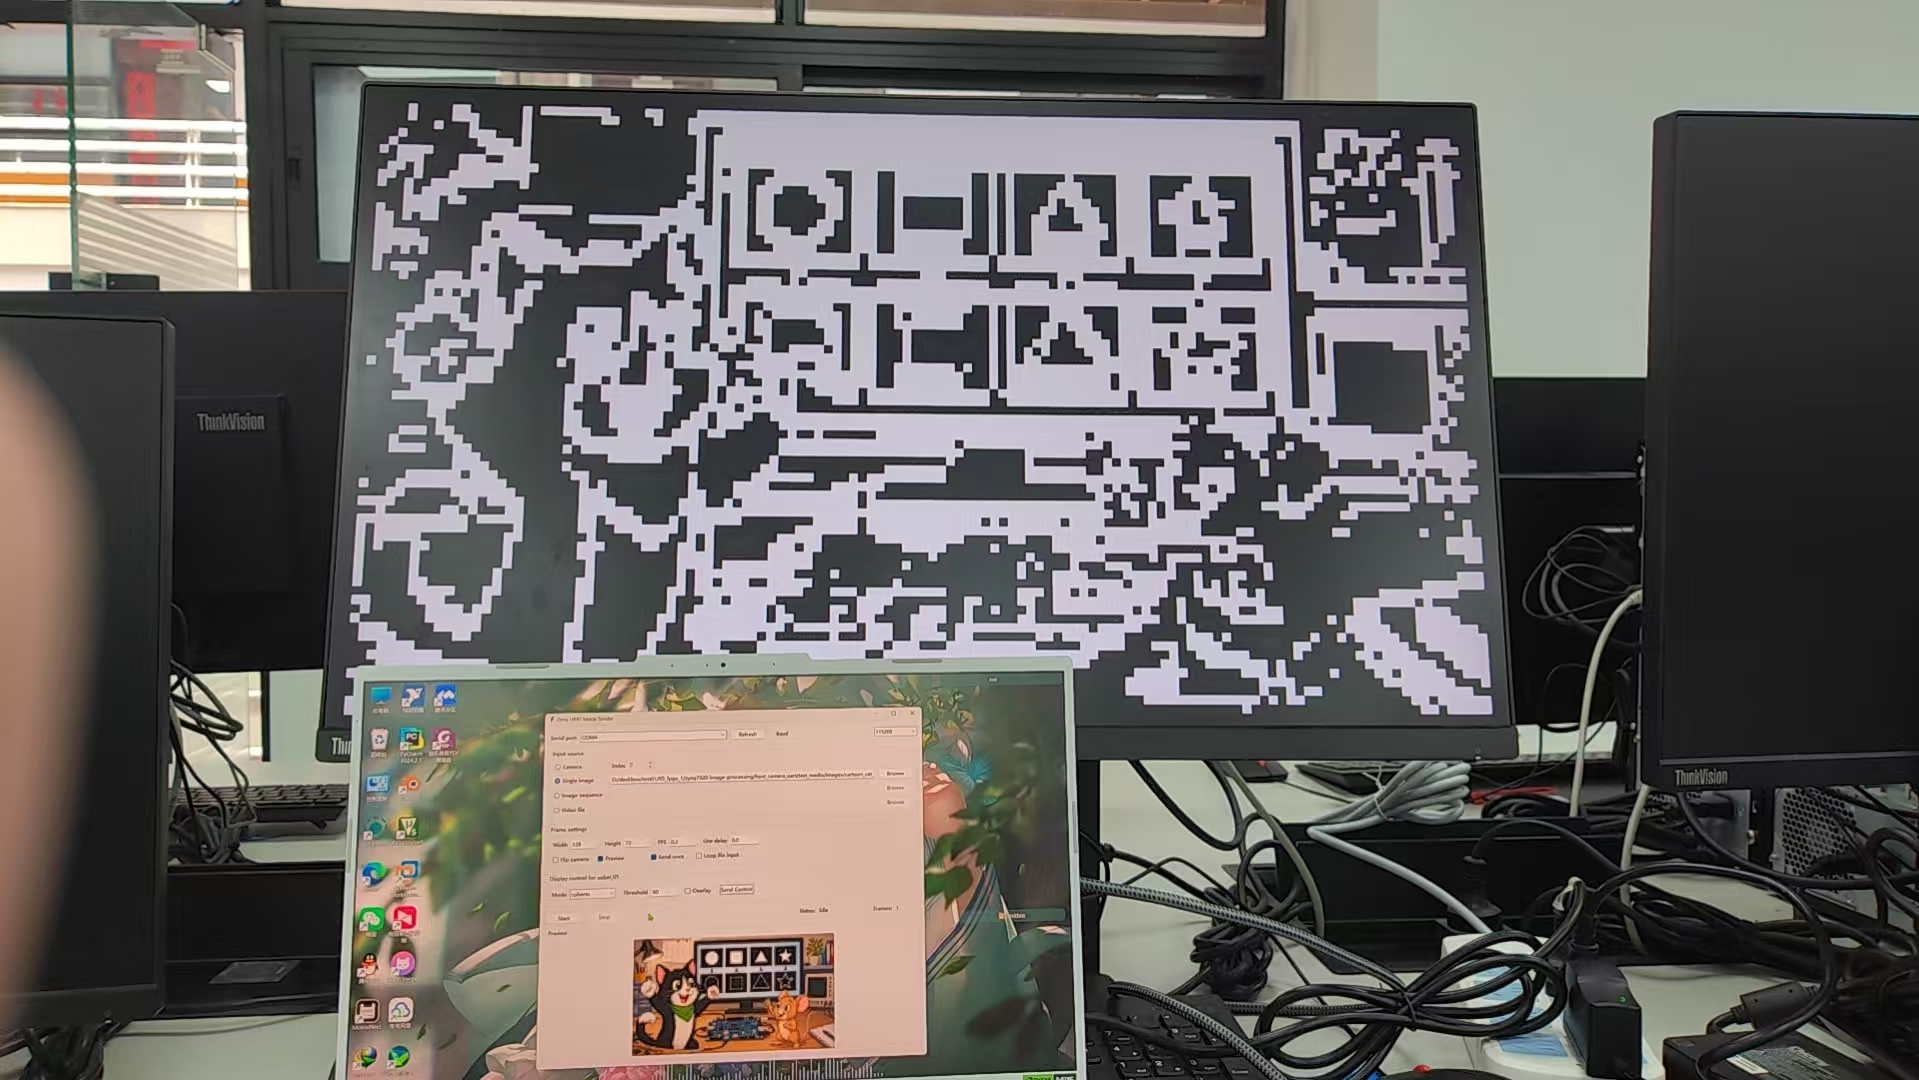
\includegraphics[width=\linewidth]{images/05扩展3/Robert_60.jpg}
        \caption{Roberts}
    \end{minipage}
    \caption{阈值60时四种算法对比}
    \label{fig:thresh60}
\end{figure}

如图\ref{fig:thresh60}所示，当阈值提高到60时，各算法检测到的边缘减少，噪声得到一定抑制。Sobel和Prewitt的边缘更加清晰，Laplacian的噪点有所减少但仍比其他算法多。这说明提高阈值可以有效抑制噪声，但也会丢失一些弱边缘信息。

\begin{figure}[H]
    \centering
    \begin{minipage}{0.48\textwidth}
        \centering
        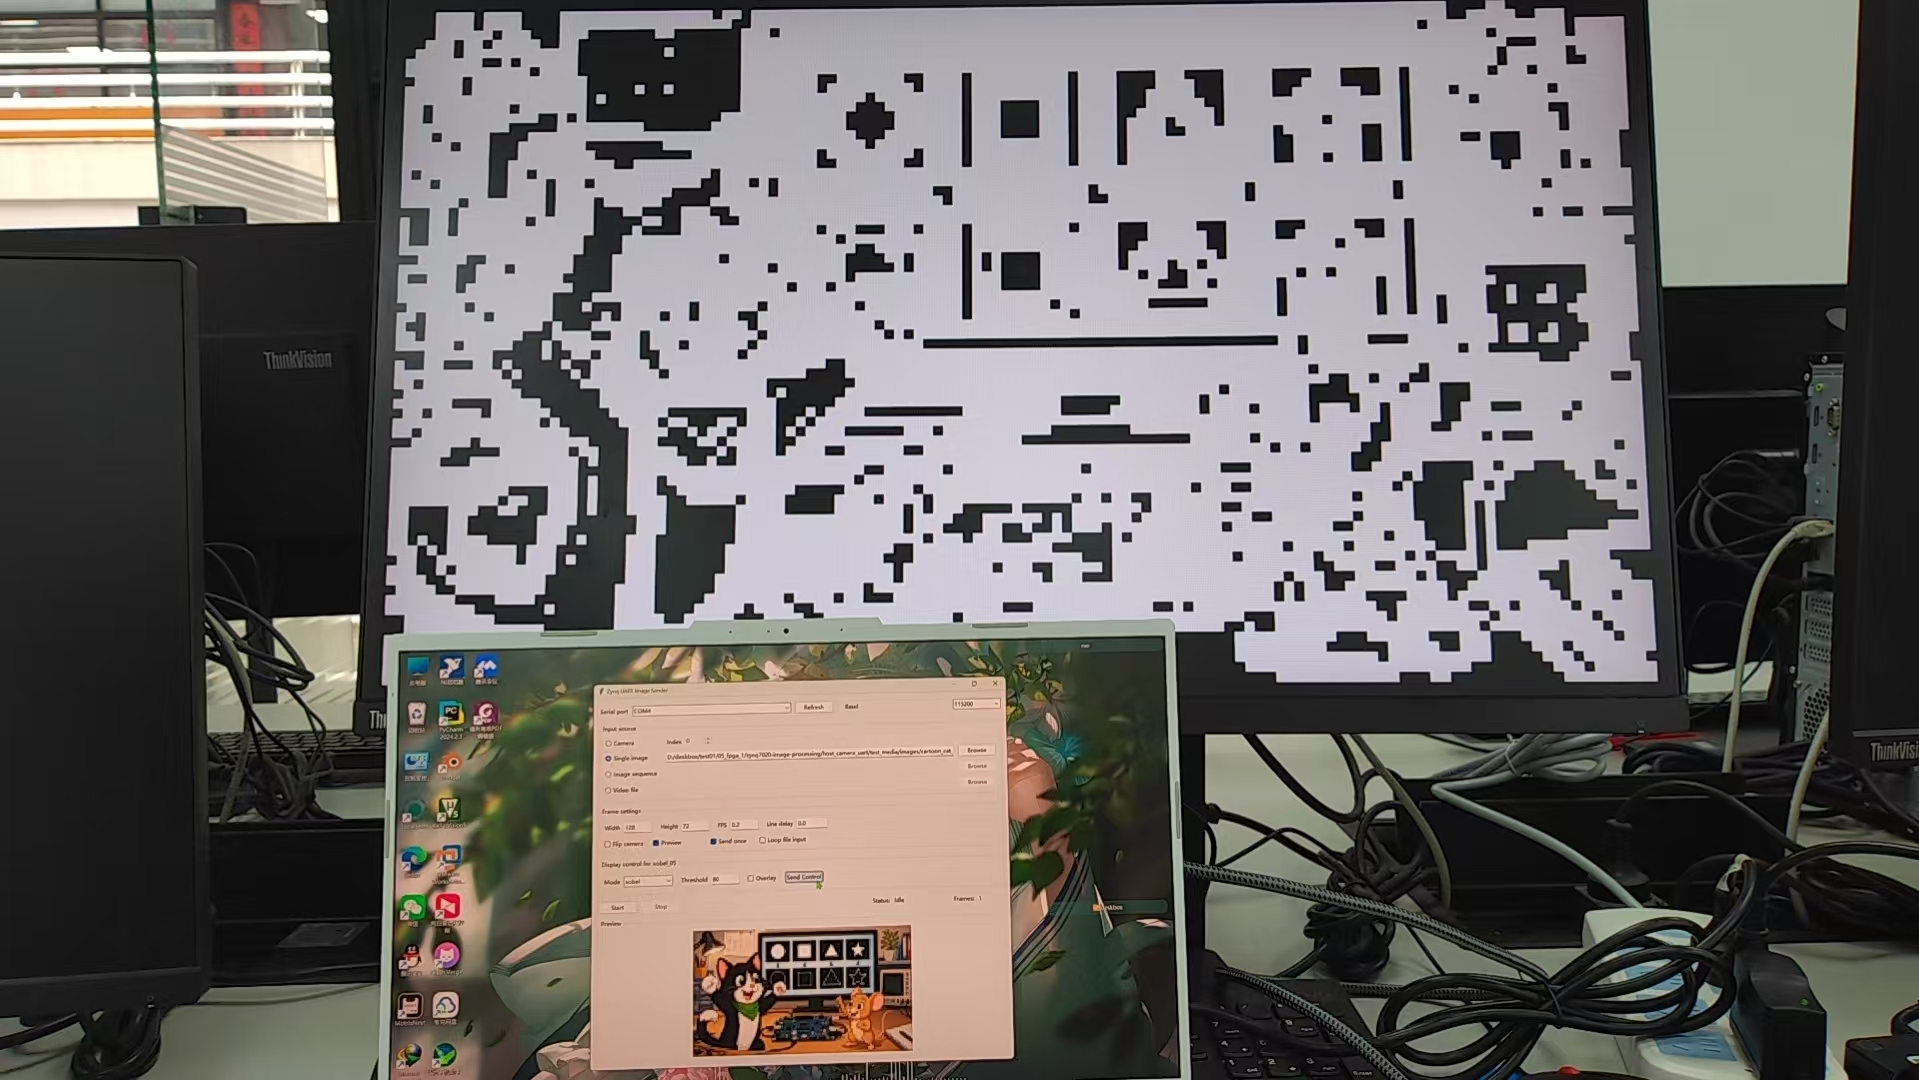
\includegraphics[width=\linewidth]{images/05扩展3/sobel_80.jpg}
        \caption{Sobel}
    \end{minipage}
    \hfill
    \begin{minipage}{0.48\textwidth}
        \centering
        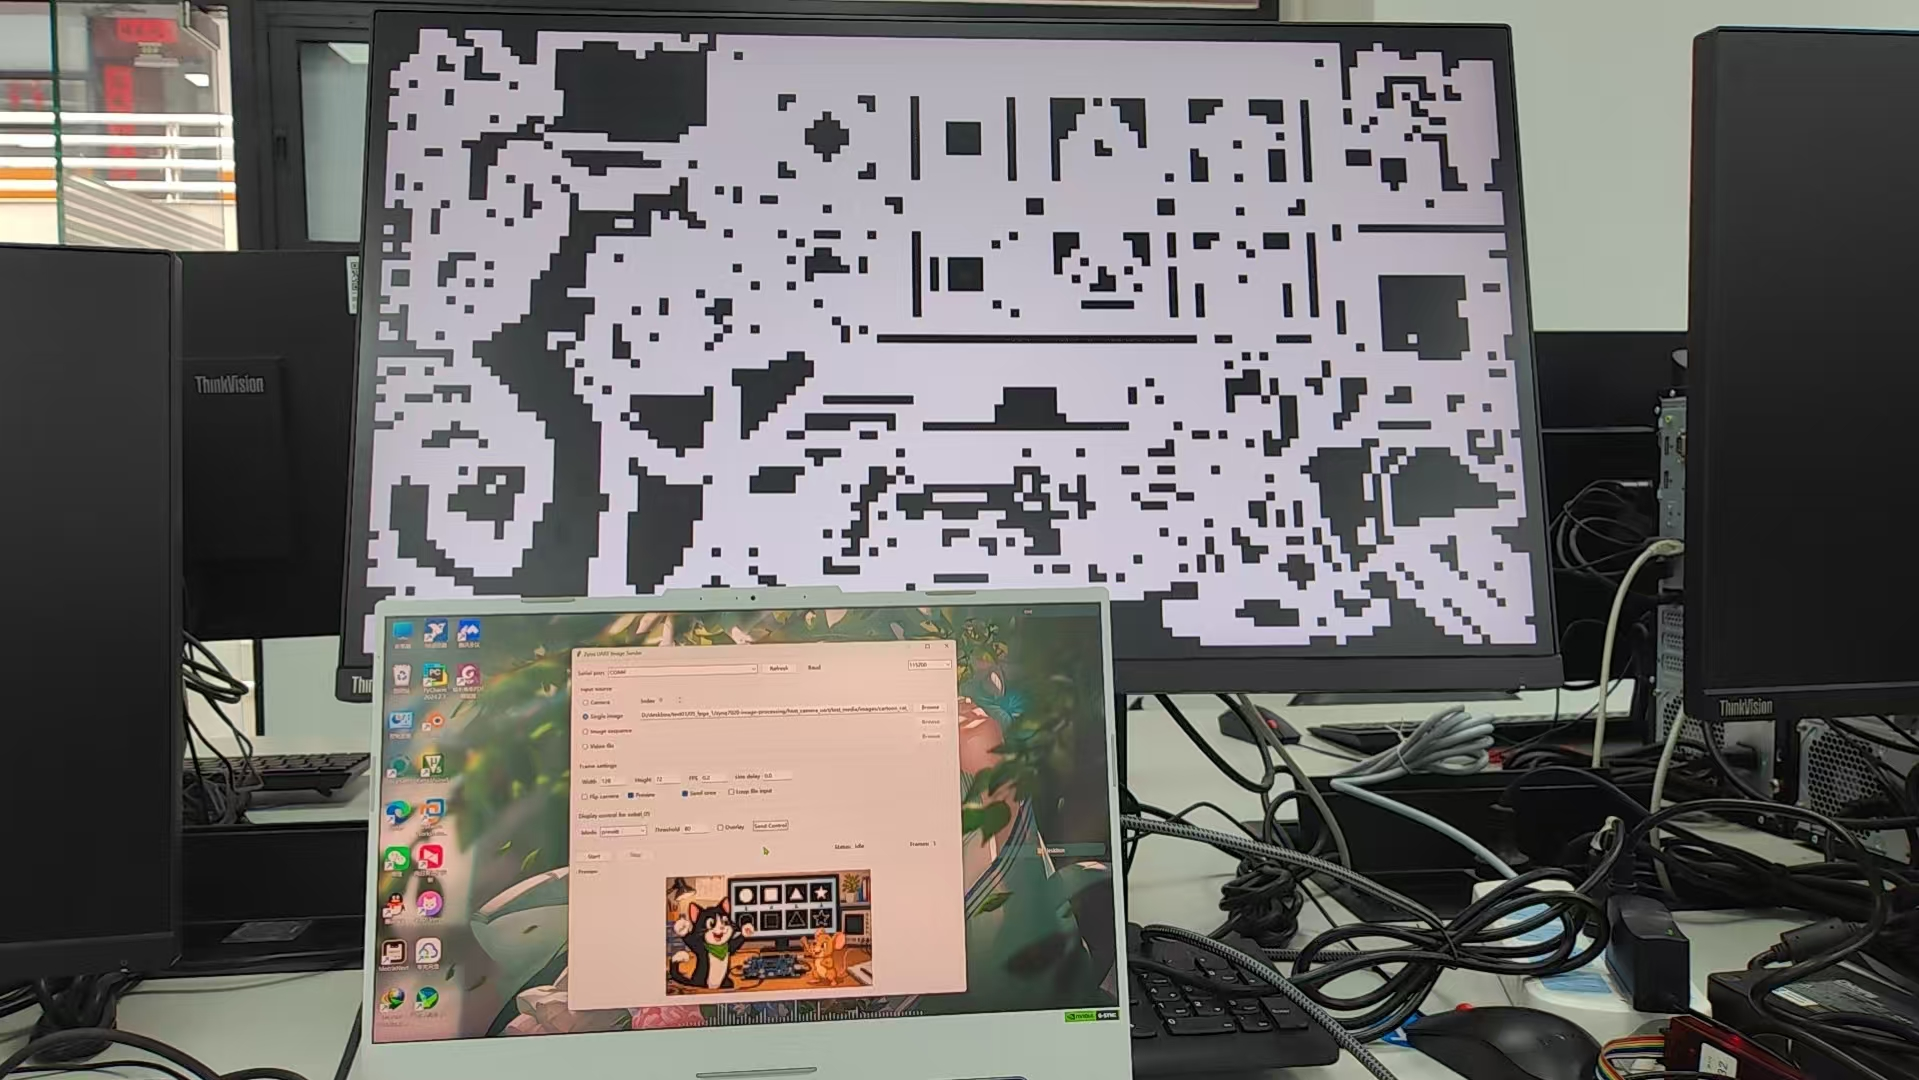
\includegraphics[width=\linewidth]{images/05扩展3/prewitt_80.jpg}
        \caption{Prewitt}
    \end{minipage}
    \par\vspace{1em}
    \begin{minipage}{0.48\textwidth}
        \centering
        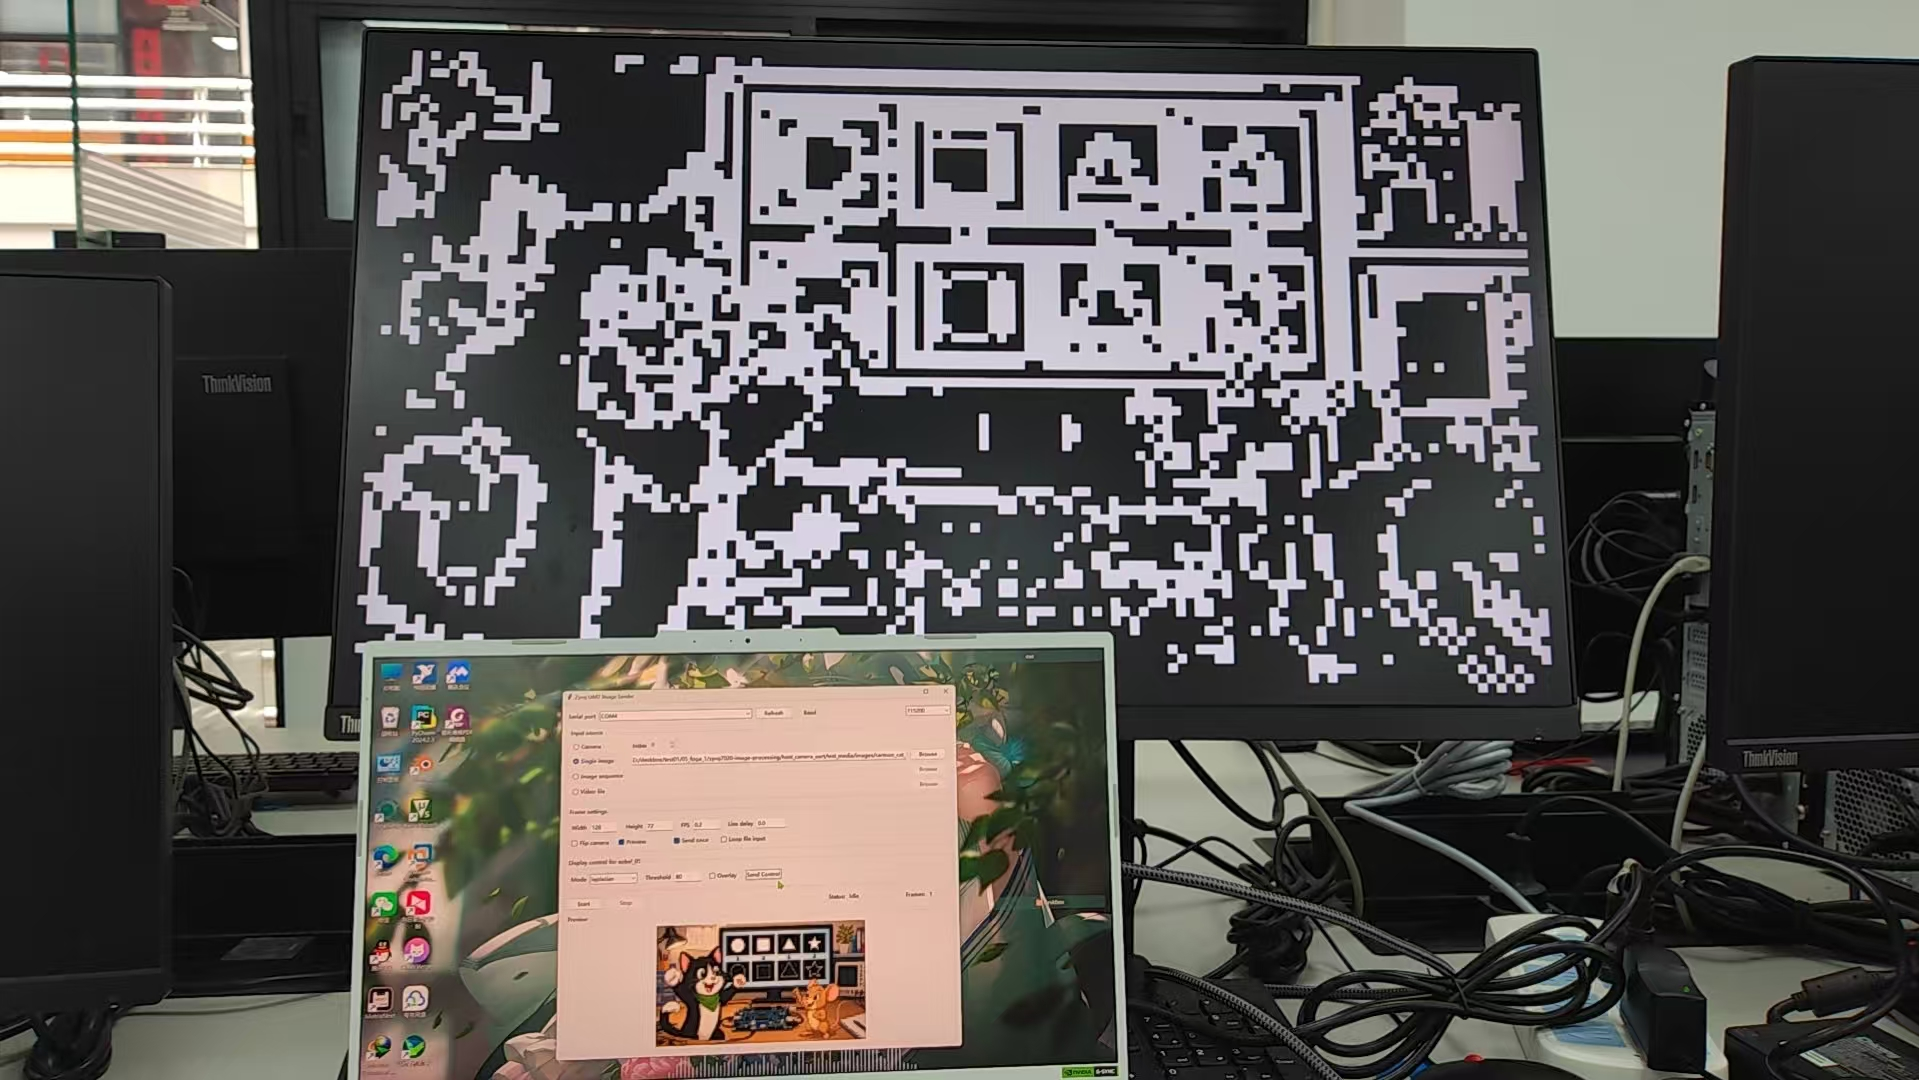
\includegraphics[width=\linewidth]{images/05扩展3/laplacian_80.jpg}
        \caption{Laplacian}
    \end{minipage}
    \hfill
    \begin{minipage}{0.48\textwidth}
        \centering
        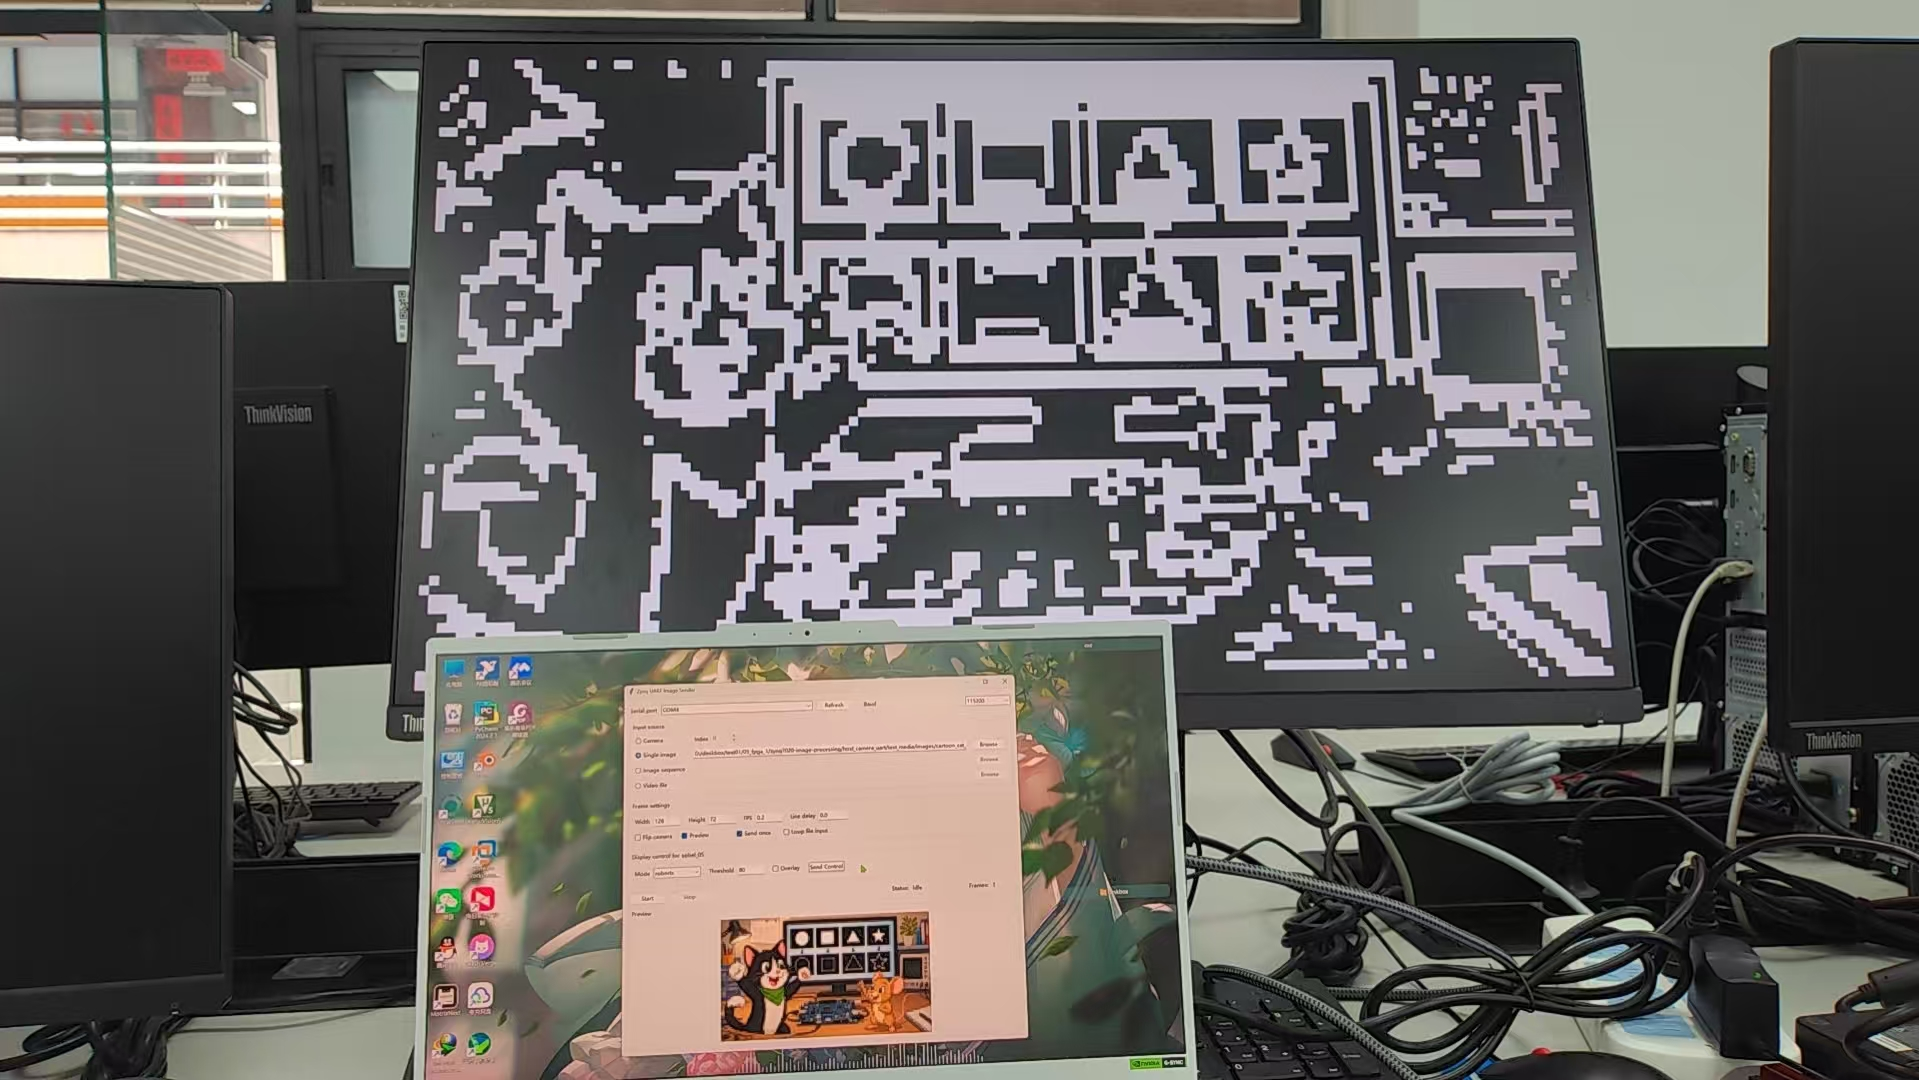
\includegraphics[width=\linewidth]{images/05扩展3/Robert_80.jpg}
        \caption{Roberts}
    \end{minipage}
    \caption{阈值80时四种算法对比}
    \label{fig:thresh80}
\end{figure}

如图\ref{fig:thresh80}所示，当阈值提高到80时，只有较强的边缘被保留。Sobel和Prewitt的边缘效果最为接近，Roberts保留了较多对角线边缘，Laplacian的边缘细节仍然最丰富。这表明在高阈值下，各算法的差异主要体现在边缘细节和噪声抑制上。

\subsubsection{资源利用率与时序结果}

Vivado综合后的资源利用率如图\ref{fig:resource}所示。新增3个算法核后，资源增量可控。Prewitt和Roberts由于不使用2x乘法，不消耗额外DSP资源；Laplacian的4倍乘法可优化为左移2位实现。四种算法共享行缓冲和灰度转换逻辑，资源利用率较高。

\begin{figure}[H]
    \centering
    
\includegraphics[width=0.9\textwidth]{images/05扩展3/资源利用率.png}
    \caption{Vivado资源利用率报告}
    \label{fig:resource}
\end{figure}

时序分析结果如图\ref{fig:timing}所示，新增三个算法模块后系统时序保持稳定，无时序违例。这得益于算法的并行架构设计，每个核独立处理，不会相互影响时序路径。

\begin{figure}[H]
    \centering
    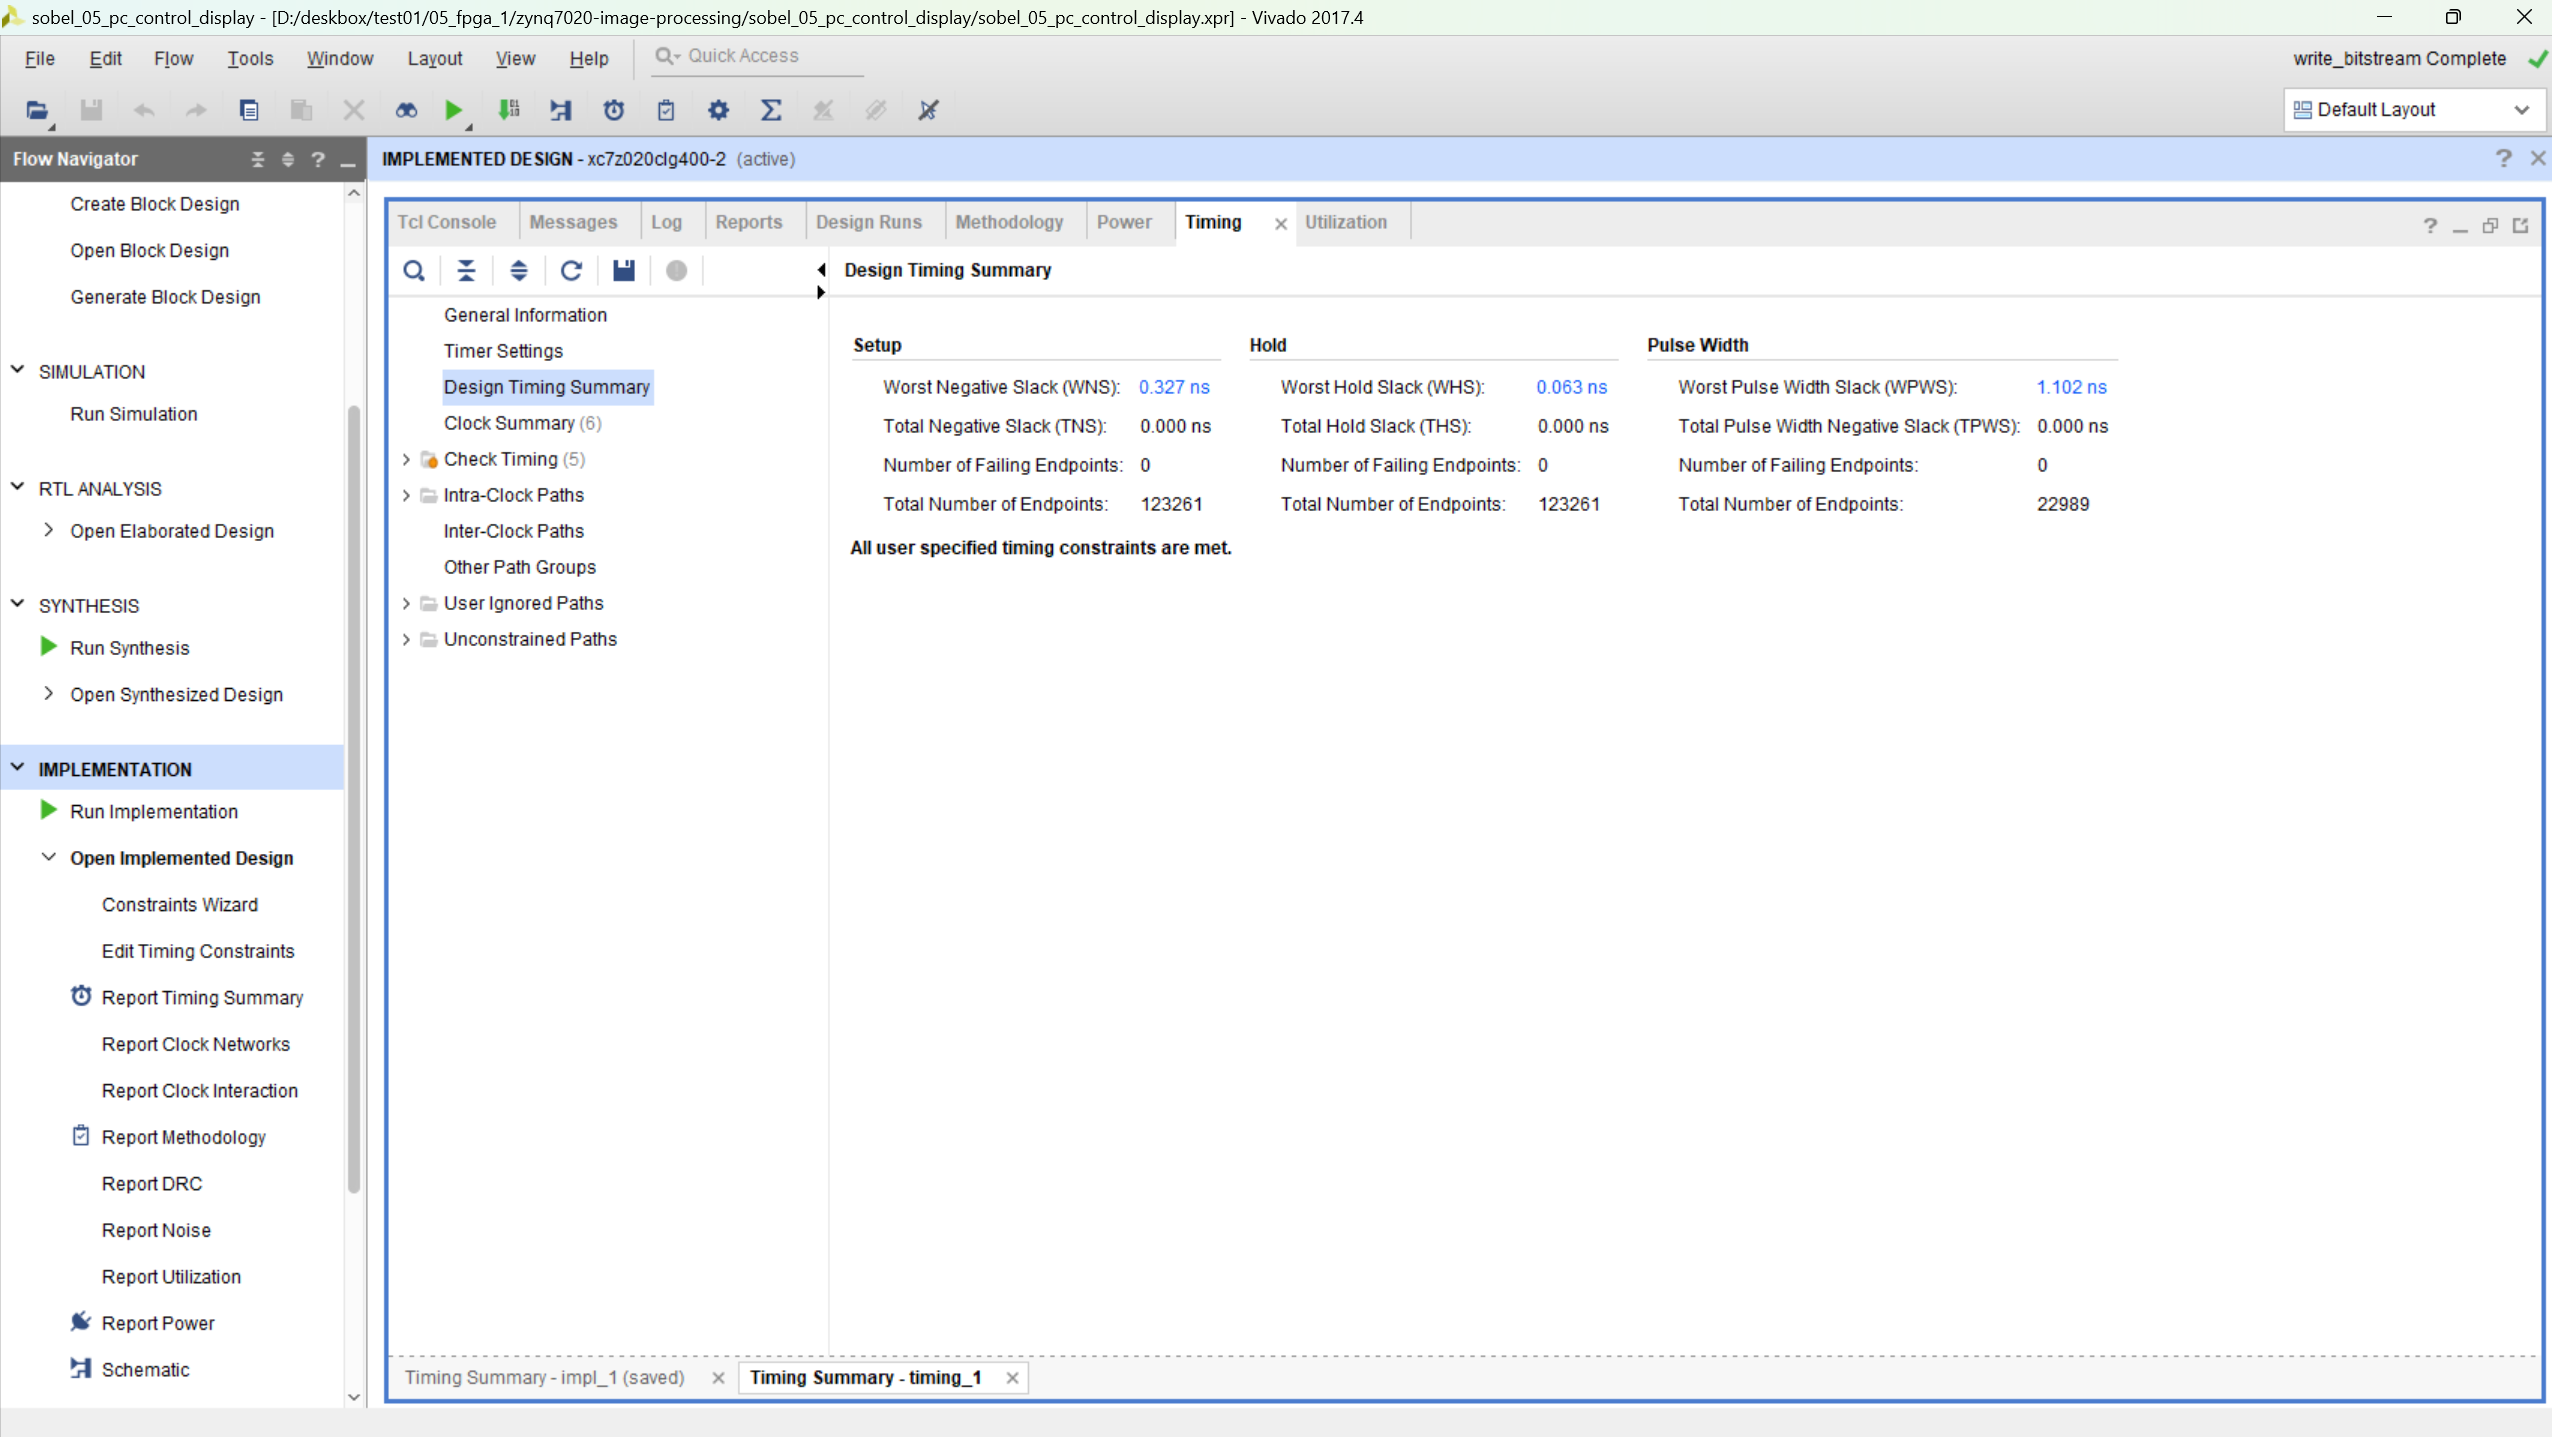
\includegraphics[width=0.9\textwidth]{images/05扩展3/时序对比分析.png}
    \caption{Vivado时序分析结果}
    \label{fig:timing}
\end{figure}

\subsubsection{上板演示现象}

上板验证结果如图\ref{fig:hw}所示，所有模式均可通过上位机命令实时切换。灰度图显示正确，Sobel边缘检测效果良好，彩色边缘叠加模式将原图与边缘叠加显示。

\begin{figure}[H]
    \centering
    \begin{minipage}{0.48\textwidth}
        \centering
        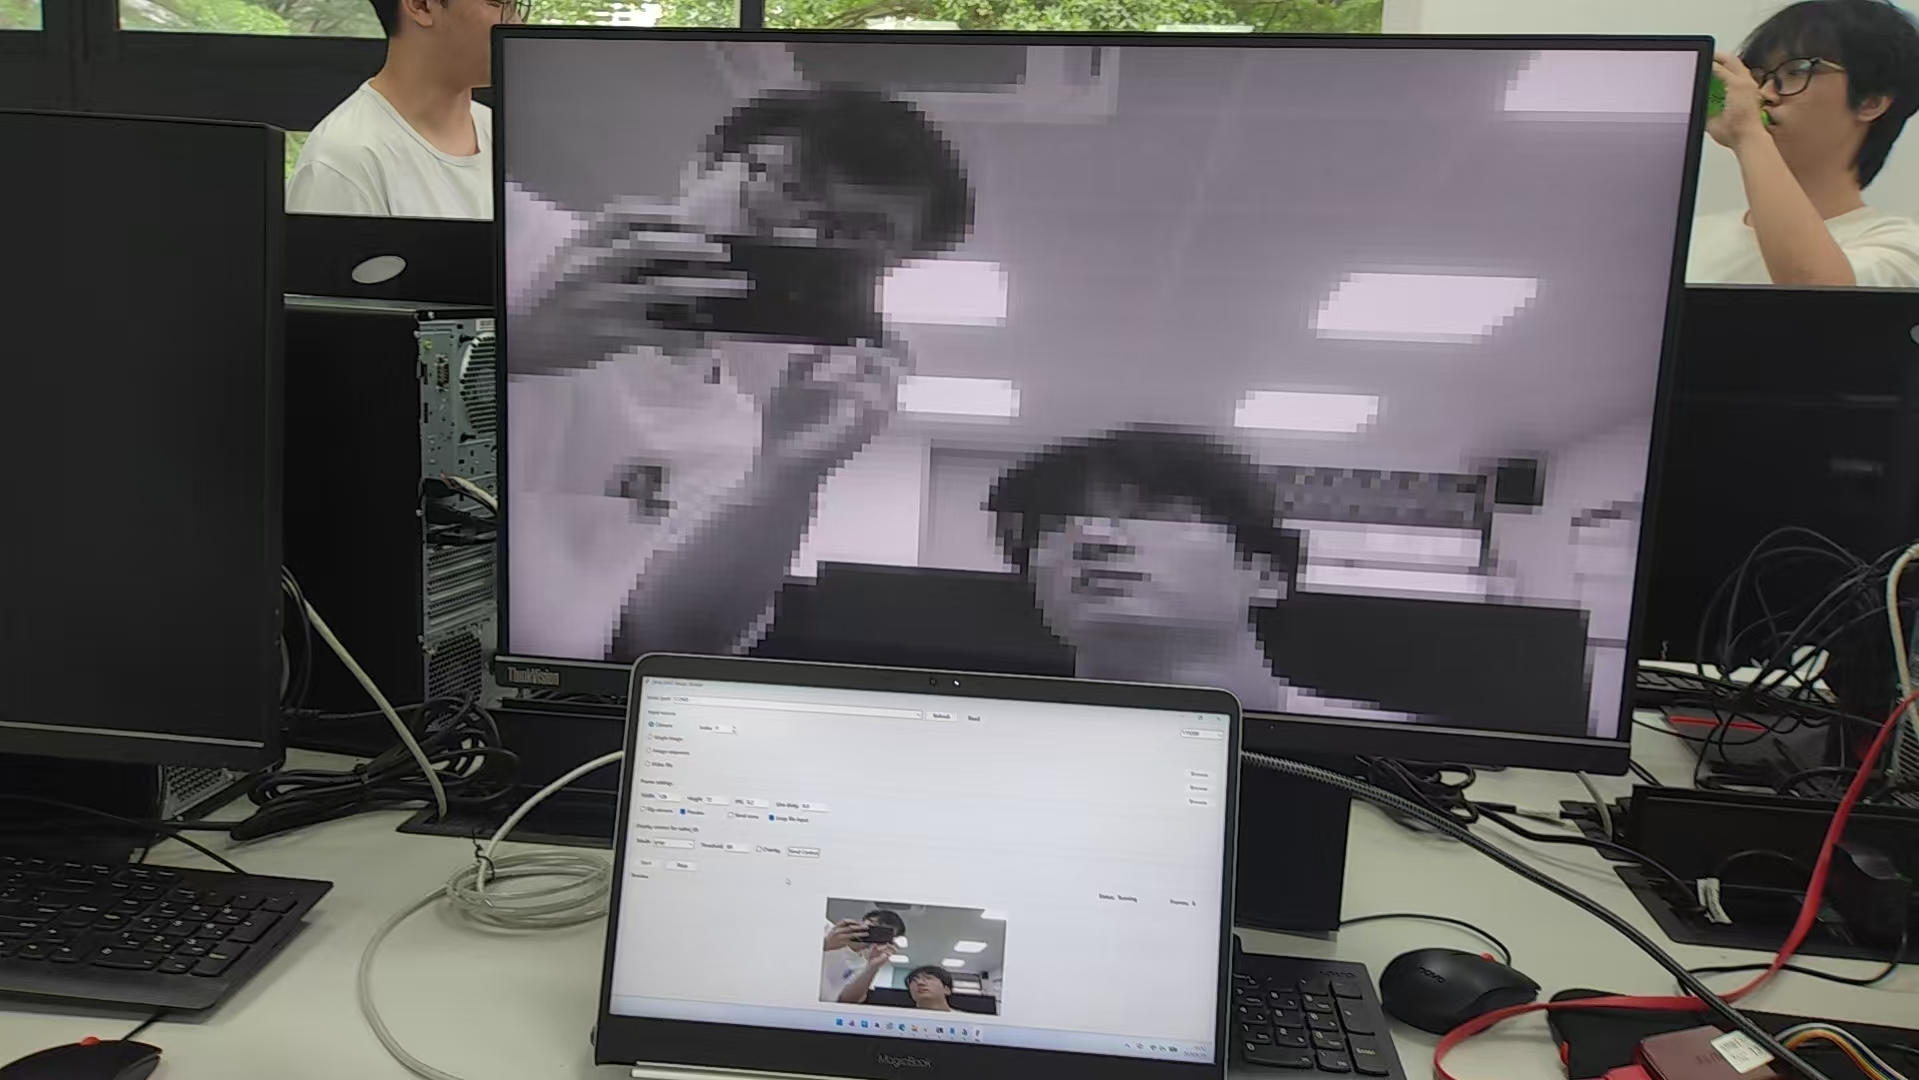
\includegraphics[width=\linewidth]{images/05/灰度图.jpg}
        \caption{灰度图显示}
    \end{minipage}
    \hfill
    \begin{minipage}{0.48\textwidth}
        \centering
        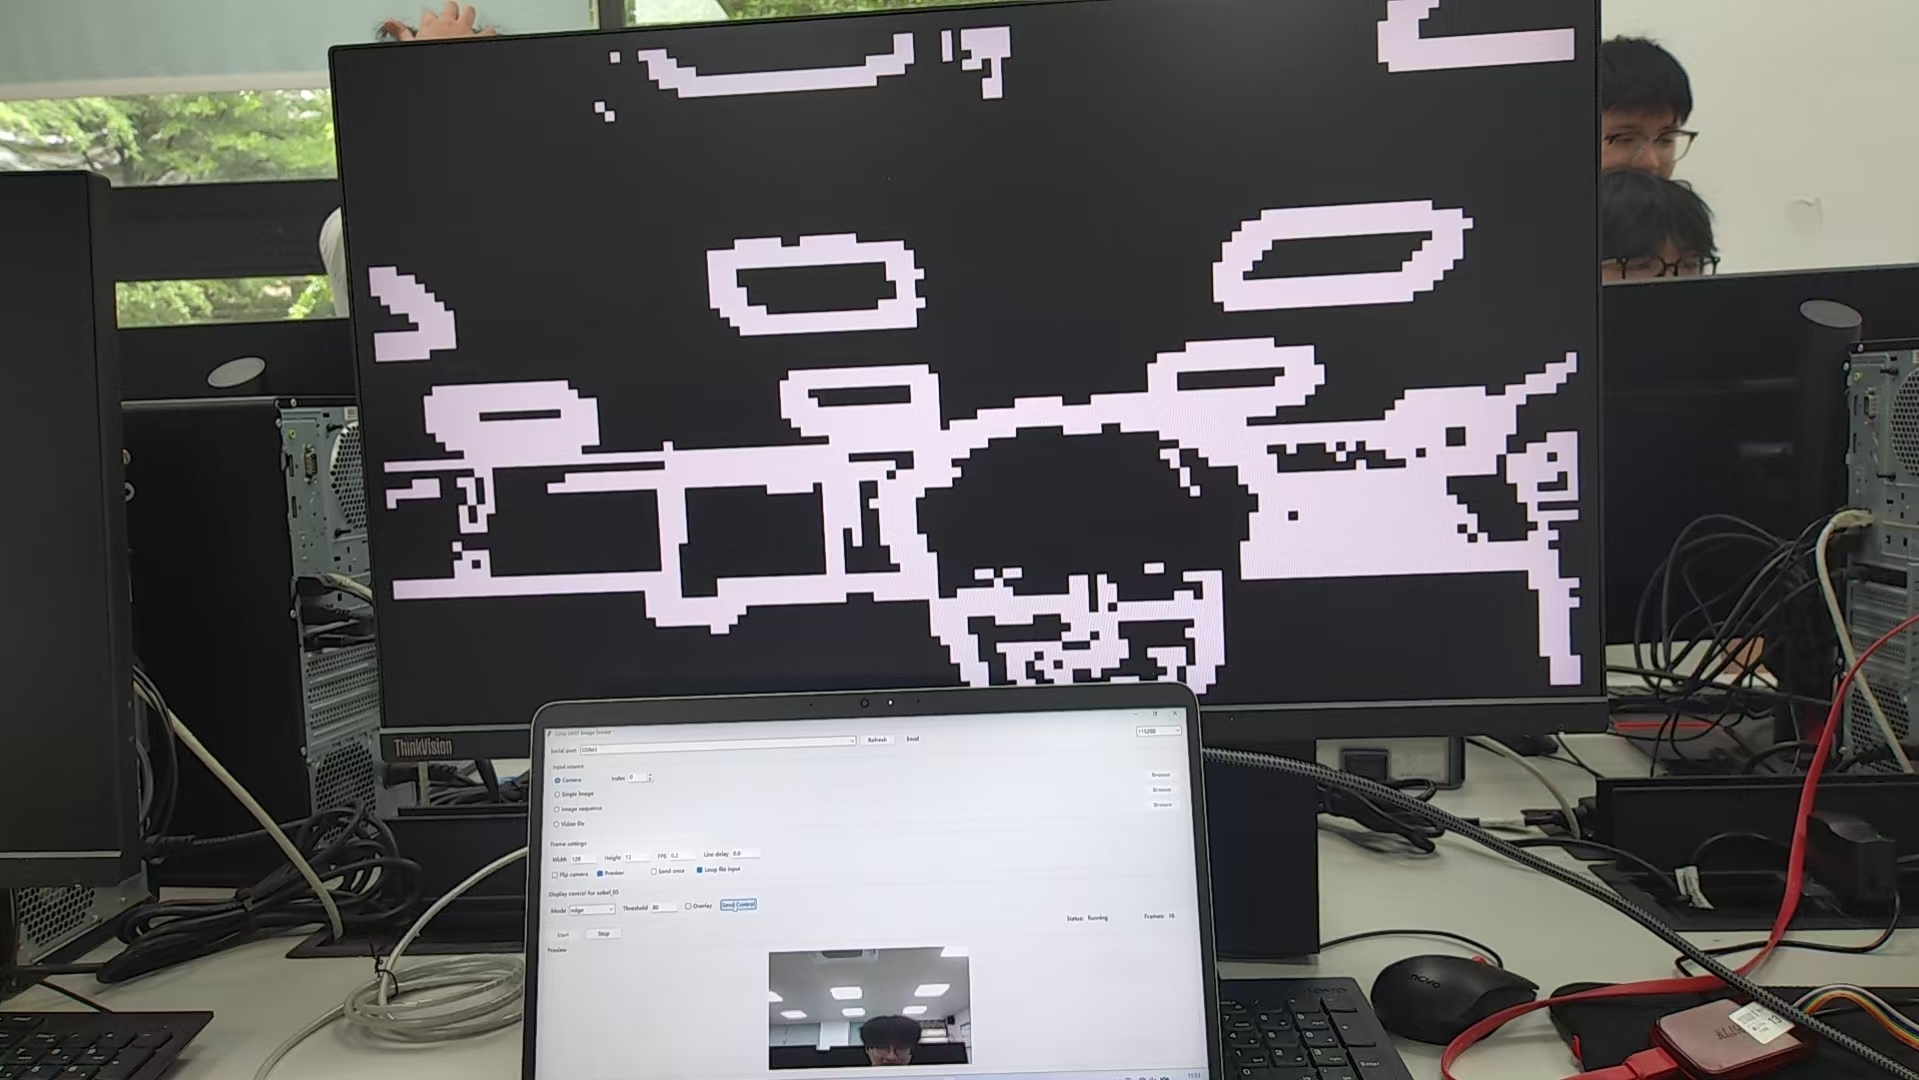
\includegraphics[width=\linewidth]{images/05/二值边缘图.jpg}
        \caption{Sobel边缘检测}
    \end{minipage}
    \par\vspace{1em}
    \begin{minipage}{0.48\textwidth}
        \centering
        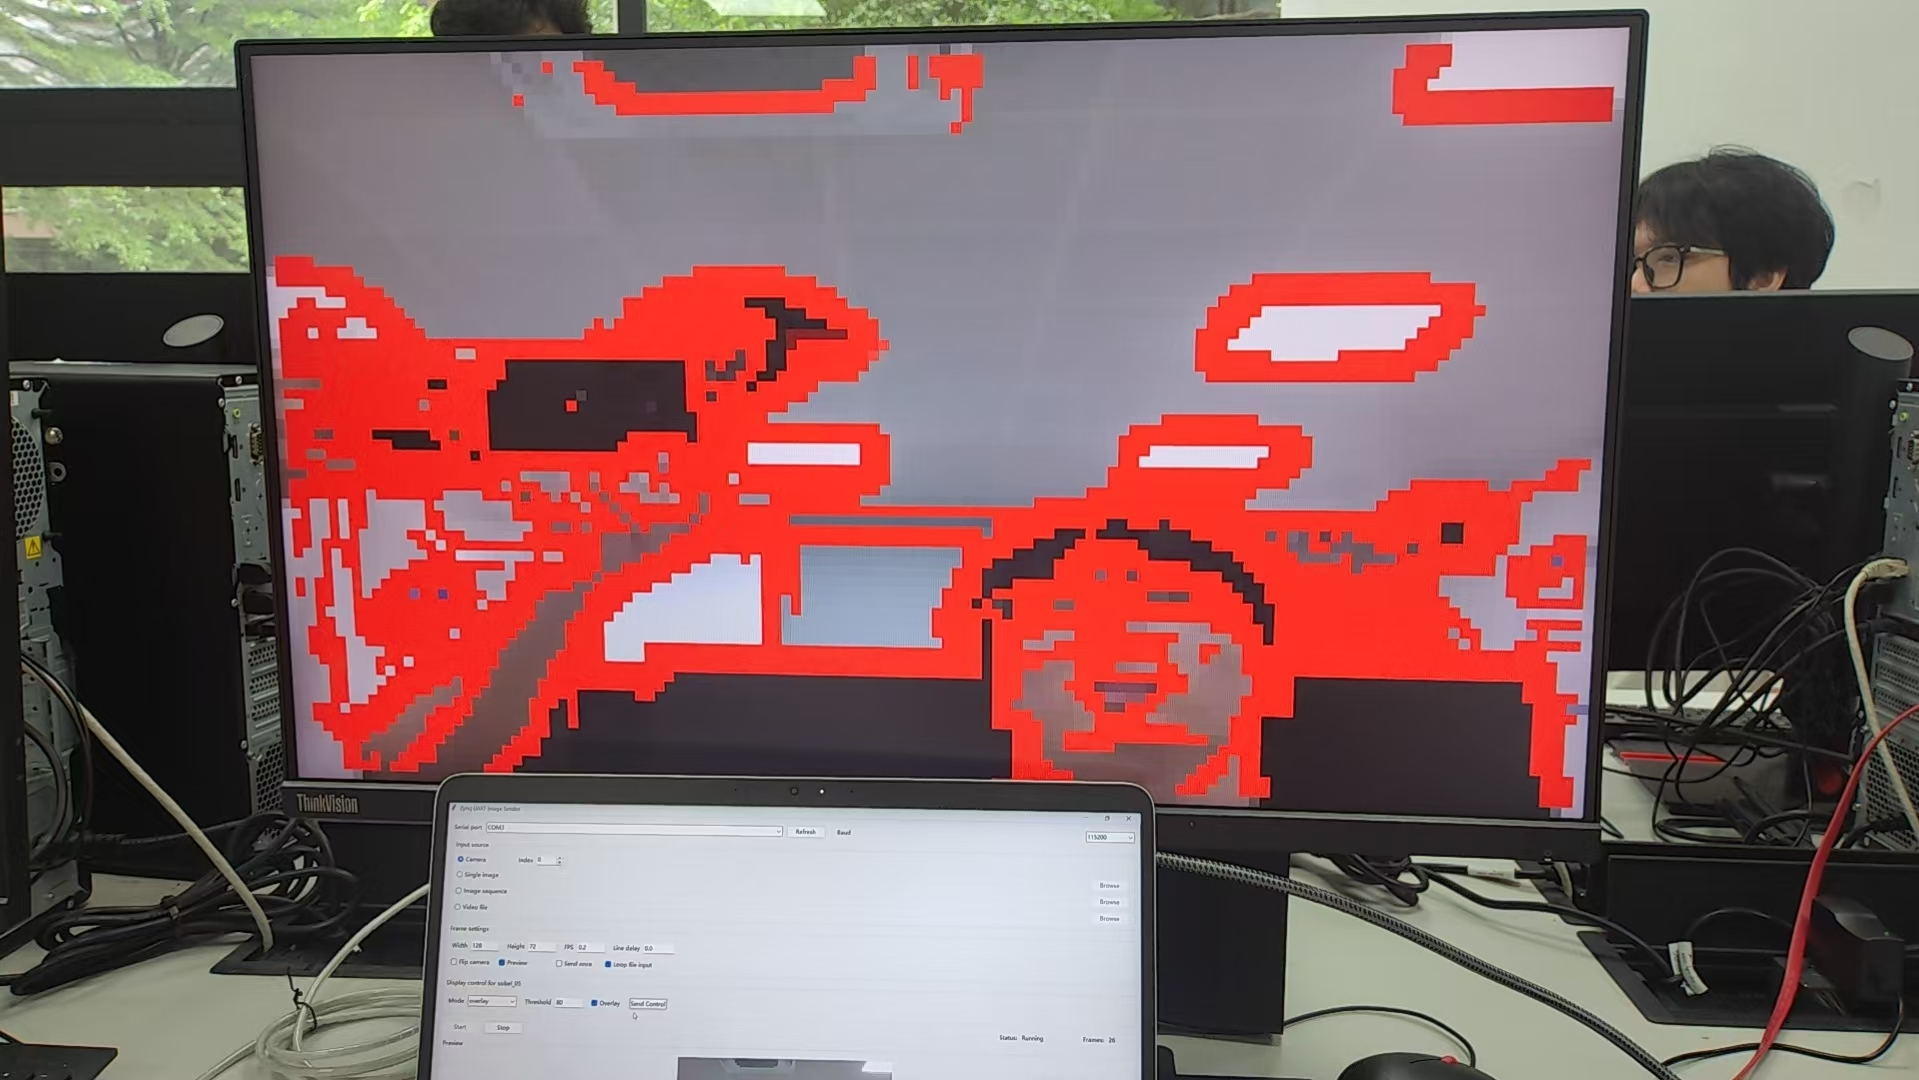
\includegraphics[width=\linewidth]{images/05/彩色边缘图.jpg}
        \caption{彩色边缘叠加}
    \end{minipage}
    \caption{上板验证结果}
    \label{fig:hw}
\end{figure}

\subsubsection{上位机控制界面}

上位机控制界面如图\ref{fig:ui}所示，支持模式切换和阈值调整。用户可通过命令A5 5A 01 04/05/06切换到Laplacian/Prewitt/Roberts模式，通过A5 5A 02 XX设置边缘二值化阈值。

\begin{figure}[H]
    \centering
    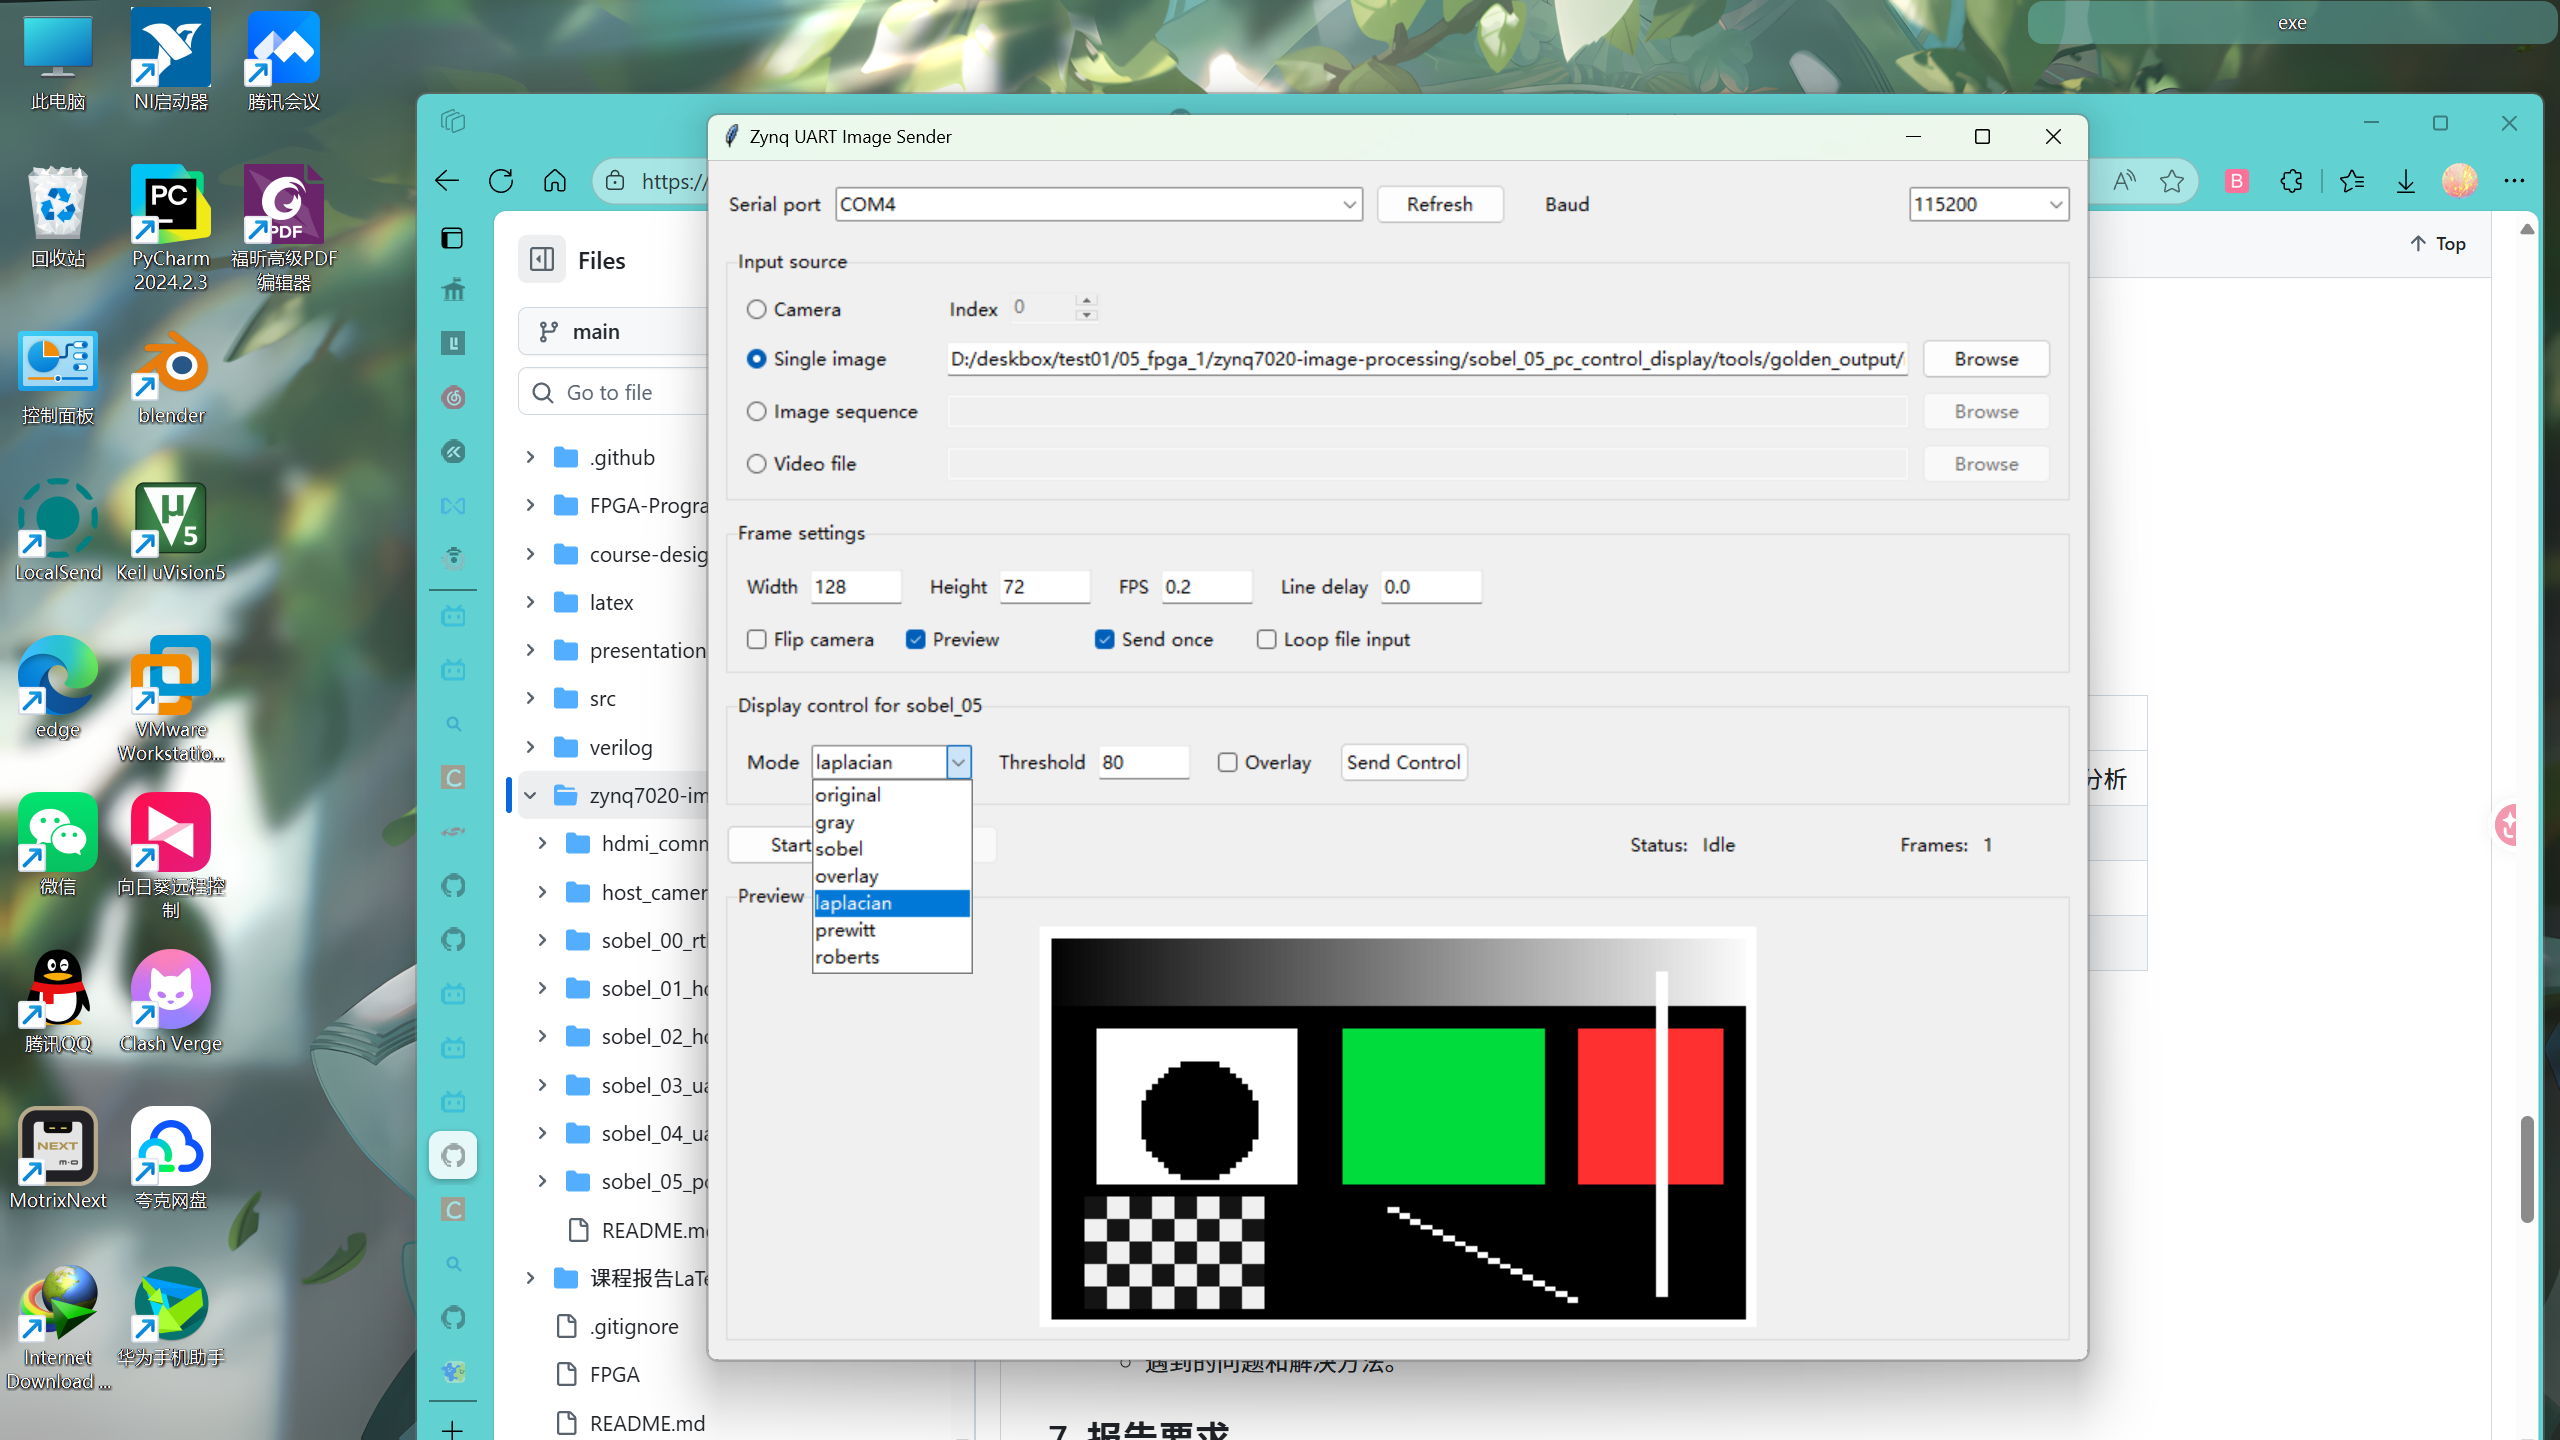
\includegraphics[width=0.9\textwidth]{images/05扩展3/上位机ui.png}
    \caption{上位机控制界面}
    \label{fig:ui}
\end{figure}
